\documentclass[a4paper,12pt]{article}
\usepackage[utf8]{inputenc}
\usepackage[ngerman]{babel}
\usepackage{geometry}
\geometry{a4paper, top=3cm, bottom=3cm, left=3.5cm, right=2.5cm}
\usepackage{setspace}
\usepackage{graphicx}
\usepackage{cite}
\usepackage{hyperref}
\usepackage{url}
\usepackage{glossaries}
\usepackage{setspace}
\onehalfspacing 
\makeglossaries

\usepackage{endnotes}
\usepackage{float} 
\usepackage{booktabs}
\usepackage{acronym}
\let\footnote=\endnote

\begin{document}
	\thispagestyle{empty}
	
	\begin{center}
		\vspace*{2cm}

		\Huge\textbf{Anomalie-Erkennung in Keycloak-Logs mittels maschinellen Lernens: Vergleich von Hybridmodellen} \\[1.5cm]
		
		\normalsize
		Vorgelegt von: \\[0.3cm]
		\textbf{Ümmühan Ay} \\
		Matrikelnummer: 7060837 \\[1cm]
		
		Eingereicht am: 24.03.2025 \\[0.3cm]
		Abgabedatum: 08.09.2025 \\[1cm]
		
		Duale Hochschule Baden-Württemberg Stuttgart\\
		Fakultät für Informatik \\[2cm]
		
		Erstprüfer: Eric Hämmerle \\
		Zweitprüfer: Dr. Janko Dietzsch
		
	\end{center}
	
	\newpage
	\section*{Abstract}
	
	\newpage
	\section*{Zusammenfassung}
	
	\newpage
	\section*{Eigenständigkeitserklärung}
	
	Hiermit erkläre ich, dass ich die vorliegende Arbeit selbstständig und ohne unzulässige fremde Hilfe angefertigt habe.  
	Alle verwendeten Quellen und Hilfsmittel sind in der Arbeit angegeben.  
	Diese Arbeit wurde bisher keiner anderen Prüfungsbehörde vorgelegt und auch nicht veröffentlicht.
	
	\vspace{2cm}
	
	\noindent Ort, Datum \hfill Unterschrift
	\newpage
	\tableofcontents
	\newpage
	\listoffigures
	\newpage
	\listoftables
	\newpage
	
	\section*{Abkürzungsverzeichnis}
	
	\textbf{ABAC:} Attribute-Based Access Control \\[1em]
	\textbf{AE:} Autoencoder \\[1em]
	\textbf{AUC-PR:} Area Under the Precision and Recall Curve \\[1em]
	\textbf{AUC-ROC:} Area Under the ROC Curve \\[1em]
	\textbf{DBSCAN:} Density-Based Spatial Clustering of Applications with Noise
	\textbf{DGX:} Deep GPU Xceleration \\[1em]
	\textbf{IAM:} Identity und Access Management \\[1em]
	\textbf{IF:} Isolation Forest \\[1em]
	\textbf{LSTM:} Long Short Term Memory \\[1em]
	\textbf{MCC:} Matthews Correlation Coefficient \\[1em]
	\textbf{MITRE ATT\&CK: } MITRE Adversarial Tactics, Techniques, 
		and Common Knowledge \\[1em]
	\textbf{ML:} Machine Learning \\[1em]
	\textbf{OCSVM:} One Class Support Vector Machine \\[1em]
	\textbf{RBAC:} Role-Based Access Control \\[1em]
	\textbf{RNN:} Recurrent Neural Network \\[1em]
	\textbf{SSO:} Single-Sign-On \\[1em]
	\textbf {UBA:} User Behavior Analytics \\[0.1em]
	\textbf {UEBA:} User and Entity Behavior Analytics \\[0.1em]
	
	\newpage
	
	\newglossaryentry{abac}{
		name={ABAC},
		description={Zugriffskontrolle basierend auf Benutzerattributen wie Rolle, Standort, Zeit etc.}
	}
	
	\newglossaryentry{aucpr}{
		name={AUC-PR},
		description={Area Under the Precision and Recall Curve – misst die Leistung eines Modells im Umgang mit unausgeglichenen Klassen.}
	}
	
	\newglossaryentry{aucroc}{
		name={AUC-ROC},
		description={Area Under the Receiver Operating Characteristic Curve – misst die Trennschärfe eines Klassifikationsmodells.}
	}
	
	\newglossaryentry{Autoencoder}{
		name={AE},
		description={Autoencoder – Neuronales Netzwerk zur komprimierten Darstellung und Rekonstruktion von Daten.}
	}
	
	\newglossaryentry{balancedaccuracy}{
		name={Balanced Accuracy},
		description={Durchschnitt aus Sensitivität (Recall) und Spezifität; besonders geeignet bei unausgeglichenen Klassenverhältnissen}
	}
	
	\newglossaryentry{clientrole}{
		name=Client-Role,
		description={Client-spezifische Rollen in Keycloak, die Zugriffsrechte innerhalb einer bestimmten Anwendung steuern}
	}
	
	\newglossaryentry{dbscan}{
		name={DBSCAN},
		description={Density-Based Spatial Clustering of Applications with Noise – Clustering-Verfahren für dichte Datenregionen.}
	}
	
	\newglossaryentry{dgx}{
		name={DGX},
		description={Deep GPU Xceleration – NVIDIA-Hardwareplattform zur KI-Beschleunigung.}
	}
	
	\newglossaryentry{hybridmodell}{
		name={Hybridmodell},
		description={Ein Modell, das zwei oder mehr unterschiedliche Verfahren kombiniert, z.\,B. LSTM-Autoencoder mit einem klassischen ML-Algorithmus wie Isolation Forest}
	}
	
	\newglossaryentry{iam}{
		name={IAM},
		description={Identity and Access Management – Verwaltung von Identitäten und Zugriffsrechten.}
	}
	
	\newglossaryentry{if}{
		name={IF},
		description={Isolation Forest – Verfahren zur Anomalieerkennung durch zufällige Isolation.}
	}
	
	\newglossaryentry{keycloak}{
		name={Keycloak},
		description={Open-Source Identity-Management-Lösung mit Funktionen wie SSO, RBAC und Brute-Force-Schutz.}
	}
	
	\newglossaryentry{lstmae}{
		name={LSTM-Autoencoder},
		description={Ein neuronales Netzwerk, das auf Long Short-Term Memory-Zellen basiert, um Sequenzen zu kodieren und zu rekonstruieren, oft zur Anomalieerkennung in Zeitreihen}
	}
	
	\newglossaryentry{lstm}{
		name={LSTM},
		description={Long Short-Term Memory – Neuronales Netz zur Verarbeitung von Sequenzdaten mit Langzeitspeicher.}
	}
	
	
	\newglossaryentry{mcc}{
		name={Matthews Correlation Coefficient (MCC)},
		description={Eine robuste Metrik, die alle Werte der Konfusionsmatrix berücksichtigt; besonders geeignet bei unausgeglichenen Datensätzen}
	}
	
	\newglossaryentry{mitreattack}{
		name={MITRE ATT\&CK},
		description={MITRE Adversarial Tactics, Techniques, and Common Knowledge – öffentliches Framework zur Kategorisierung von Angriffstechniken.}
	}
	
	\newglossaryentry{ml}{
		name={ML},
		description={Machine Learning – Teilgebiet der KI, bei dem Systeme aus Daten lernen.}
	}
	
	\newglossaryentry{ocsvm}{
		name={OCSVM},
		description={One-Class Support Vector Machine – Algorithmus zur Anomalieerkennung mit einseitiger Klassifikation.}
	}
	
	\newglossaryentry{rbac}{
		name={RBAC},
		description={Role-Based Access Control – Zugriffskontrolle auf Basis definierter Rollen.}
	}
	
	\newglossaryentry{realmrole}{
		name=Realm-Role,
		description={Globale Rollen in Keycloak, die auf alle Clients eines Realms angewendet werden können}
	}
	
	\newglossaryentry{rnn}{
		name={RNN},
		description={Recurrent Neural Network – Neuronales Netz zur Verarbeitung zeitabhängiger Daten.}
	}
	
	\newglossaryentry{scikit}{
		name=Scikit-learn,
		description={Eine weit verbreitete Python-Bibliothek für maschinelles Lernen mit Tools für Klassifikation, Regression, Clustering und Modellbewertung}
	}
	
	\newglossaryentry{sso}{
		name={SSO},
		description={Single Sign-On – Einmalige Authentifizierung für den Zugriff auf mehrere Anwendungen.}
	}
	
	\newglossaryentry{zerodayangriff}{
		name={Zero-Day-Angriff},
		description={Angriff auf eine bislang unbekannte Sicherheitslücke, für die noch kein Patch existiert.}
	}
	
	}
	\newglossaryentry{uba}{
		name={UBA},
		description={User Behavior Analytics – Analyse des Benutzerverhaltens zur Erkennung von Anomalien und Sicherheitsbedrohungen.}
	}
	
	\newglossaryentry{bruteforce}{
		name={Brute-Force-Angriff},
		description={Angriffsmethode, bei der Passwörter oder Zugangsdaten durch systematisches Ausprobieren aller möglichen Kombinationen erraten werden.}
	}
	
	\newglossaryentry{insiderthreat}{
		name={Insider Threat},
		description={Sicherheitsbedrohung, die von Personen innerhalb einer Organisation ausgeht, z.\,B. durch missbräuchliches Verhalten von Mitarbeitenden mit legitimen Zugriffsrechten.}
	}
	
	\newglossaryentry{botnetz}{
		name={Botnetz},
		description={Ein Zusammenschluss kompromittierter Geräte (Bots), die ferngesteuert werden, oft zur Durchführung koordinierter Angriffe wie DDoS oder zur Verbreitung von Malware.}
	}
	
	\newglossaryentry{spoofing}{
		name={Spoofing},
		description={Täuschungstechniken, bei denen sich ein Angreifer als vertrauenswürdige Instanz ausgibt, um Zugang zu Informationen oder Systemen zu erlangen.}
	}
	
	\newglossaryentry{ddos}{
		name={DDoS},
		description={Distributed Denial of Service – ein Angriff, bei dem viele Systeme gleichzeitig eine Zielressource mit Anfragen überfluten, um sie unzugänglich zu machen.}
	}
	
	\newglossaryentry{ueba}{
		name={UEBA},
		description={User and Entity Behavior Analytics – Verfahren zur Analyse des Verhaltens von Benutzern und technischen Entitäten mit dem Ziel, sicherheitsrelevante Anomalien zu identifizieren.}
	}
	
	
	\newpage
	\section{Keycloak Terme}
	
	\newglossaryentry{realm}{
		name={Realm},
		description={Isolierte Umgebung in Keycloak, in der Benutzer, Rollen und Clients separat verwaltet werden.}
	}
	
	\newglossaryentry{client}{
		name={Client},
		description={Anwendung oder Dienst, der Keycloak zur Authentifizierung und Autorisierung verwendet.}
	}
	
	\newglossaryentry{idp}{
		name={Identity Provider (IdP)},
		description={Externer Anbieter, der Authentifizierungsdienste bereitstellt (z.\,B. Google, Microsoft).}
	}
	
	\newglossaryentry{oidc}{
		name={OpenID Connect (OIDC)},
		description={Auth-Protokoll, das auf OAuth 2.0 basiert und die Identität von Nutzern sicher überträgt.}
	}
	
	\newglossaryentry{saml}{
		name={SAML},
		description={Security Assertion Markup Language – XML-basiertes Protokoll für Authentifizierung und Autorisierung.}
	}
	
	\newglossaryentry{oauth}{
		name={OAuth 2.0},
		description={Autorisierungs-Framework, das sicheren Zugriff auf geschützte Ressourcen ermöglicht.}
	}
	
	\newglossaryentry{granttype}{
		name={Grant Type},
		description={Verfahren, mit dem ein Client oder Benutzer bei einem Authentifizierungsserver ein Token anfordert.}
	}
	
	\newglossaryentry{authflow}{
		name={Authentication Flow},
		description={Ablauf, der festlegt, wie sich Benutzer oder Clients bei Keycloak authentifizieren.}
	}
	
	\newglossaryentry{clientcredentials}{
		name={Client Credentials Grant},
		description={OAuth2-Grant-Typ, bei dem sich ein Client ohne Benutzerinteraktion authentifiziert.}
	}
	
	\newglossaryentry{authcodegrant}{
		name={Authorization Code Grant},
		description={OAuth2-Grant-Typ, bei dem der Benutzer über einen Code authentifiziert wird, der vom Client gegen ein Token eingetauscht wird.}
	}
	
	\newglossaryentry{clientscope}{
		name={Client-Scope},
		description={Legt fest, welche Benutzerdaten in ein Token aufgenommen werden, wenn sich ein Benutzer über einen Client authentifiziert.}
	}
	
	\newglossaryentry{serviceaccount}{
		name={Service Account},
		description={Konto, das einem Client gehört und ohne Benutzerinteraktion für automatisierte Vorgänge eingesetzt wird.}
	}
	
	
	\printglossaries 
	\newpage

	\section{Einleitung}
	Laut dem BSI-Lagebericht 2024 ist die Zahl von Cyberangriffen auf Unternehmen durch Ransomware und DDoS-Attacken weiter gestiegen \cite{bsi2024lage}.
	Angreifende entwickeln kontinuierlich neue Methoden, um Sicherheitsmechanismen zu umgehen und finanzielle oder strategische Vorteile zu erlangen. Herkömmliche, regelbasierte Schutzmaßnahmen – etwa Firewalls oder Brute-Force-Abwehrsysteme – stoßen dabei zunehmend an ihre Grenzen.
	Besonders schwer zu erkennen sind interne Angreifer, also etwa eigene Mitarbeitende, sowie koordinierte Attacken über Botnetze. Solche Bedrohungen erfordern fortschrittliche Verfahren zur Mustererkennung. Der Einsatz von Künstlicher Intelligenz (KI) in Sicherheitssystemen gewinnt daher zunehmend an Bedeutung. Maschinelle Lernalgorithmen bieten hier ein vielversprechendes Potenzial: Sie können Anomalien identifizieren und das Nutzerverhalten auf Basis theoretischer Modelle analysieren, um Angriffe frühzeitig zu erkennen.
	
	\subsection{Benutzerverhalten und Anomalien}
	
	Das Benutzerverhalten umfasst sämtliche Aktionen, Muster und Gewohnheiten, mit denen ein Nutzer ein IT-System verwendet. Dazu zählen unter anderem Login-Zeiten, Zugriffsrechte, genutzte Ressourcen, Netzwerkbewegungen sowie Interaktionen mit Anwendungen und Daten. Die Analyse des Benutzerverhaltens dient dazu, typische Nutzungsmuster zu identifizieren und Abweichungen (sogenannte Anomalien) zu erkennen, die auf Sicherheitsvorfälle oder Missbrauch hindeuten können.
	\\[0.5em]
	Anomalien bezeichnen Datenmuster, die signifikant von erwarteten oder üblichen Verhaltensweisen abweichen. Mathematisch gesehen, ist eine Anomalie, ein abweichender Punkt vom "normalen" Bereich N1 und N2 \cite{chandola2009anomaly}. Sie können beispielsweise im Netzwerkverkehr, in eingebetteten Systemen oder anderen datenverarbeitenden Bereichen auftreten. Solche Abweichungen deuten häufig auf Systemangriffe oder technische Störungen hin.
	\\[0.5em]
	Neben systemweiten Anomalien – etwa im Netzwerkverkehr oder bei Gerätezuständen – gewinnen zunehmend benutzerbasierte Auffälligkeiten an Bedeutung.
	Systemweite Anomalien betreffen technische Parameter und Prozesse im gesamten System, wie etwa plötzliche Veränderungen im Datenverkehr, unerwartete Systemlast oder ungewöhnliche Netzwerkverbindungen \cite{chandola2009anomaly}.
	Benutzerbasierte Anomalien hingegen beziehen sich auf das individuelle Verhalten einzelner Nutzer.
	
	\subsection{Kategorisierung von Anomalien}
	Nach \cite{chandola2009anomaly} werden Anomalien in drei Hauptkategorien eingeteilt:
	
	\begin{itemize}
		\item \textbf{Punkt-Anomalien:} Einzelne Dateninstanzen, die im Vergleich zum Großteil der Daten als anomal gelten. Beispiel: Eine Kreditkartentransaktion, deren Betrag deutlich höher ist als die sonst üblichen Ausgaben einer Person.
		\item \textbf{Kontextuelle Anomalien:} Dateninstanzen, die nur in einem spezifischen Kontext als anomal betrachtet werden, ansonsten jedoch normal sind. Der Kontext wird durch sogenannte \emph{kontextuelle Attribute} definiert, z. B. Zeit oder Ort. Die \emph{verhaltensbezogenen Attribute} beschreiben die eigentlichen Eigenschaften der Dateninstanz. Beispielsweise kann eine Temperatur in einem bestimmten Gebiet im Winter als anomal gelten, im Sommer aber normal sein.
		\item \textbf{Kollektive Anomalien:} Gruppen von Datenpunkten, die zusammen eine Anomalie darstellen, obwohl einzelne Punkte für sich genommen normal erscheinen.
	\end{itemize}

	Dabei umfassen kontextuelle Anomalien zwei Arten von Attributen:
	
	\begin{enumerate}
		\item \textbf{Kontextuelle Attribute:} Bestimmen den Kontext, z. B. geografische Lage oder Zeitstempel.
		\item \textbf{Verhaltensbezogene Attribute:} Beschreiben das tatsächliche Verhalten oder die Charakteristik der Dateninstanz, z. B. die gemessene Temperatur oder der Betrag einer Transaktion.
	\end{enumerate}
	Obwohl zahlreiche Arbeiten im Bereich der Anomalieerkennung im Nutzerverhalten existieren, fehlt es an einer klaren und systematischen Definition dessen, was genau eine verhaltensbasierte Anomalie konstituiert. Stattdessen werden in der Regel Beispiele genannt, ohne dass diese in ein konsistentes semantisches Modell eingebettet werden. Diese Forschungslücke erschwert die Evaluation und Vergleichbarkeit von Verfahren erheblich – und wird auch in dieser Arbeit als Ausgangspunkt einer kritischen Einordnung aufgegriffen.
	\\[0.5em]
	Es wird davon ausgegangen, dass Anomalien welche sich im Benutzerverhalten (Verhaltensbezogene Anomalien) äußern, unter anderem folgende sein können:
	
	\begin{itemize}
		\item ungewöhnliche Login-Zeiten,
		\item verdächtige Standorte,
		\item auffällige Rollenprofile,
		\item unübliche Zugriffsrechte,
		\item eine Häufung von Anmelde- oder Autorisierungsfehlern.
	\end{itemize}
	Ein Benutzer, welcher sich Mitternachts außerhalb der üblichen Geschäftszeit einloggt, ist ungewöhnlich und weicht vom gewöhnlichen Muster ab. Zudem ist es eher so, dass Arbeiter in der Region bleiben, wo sie arbeiten oder im Umkreis. Natürlich muss man hier moderne Szenarien beachten, z.B. tritt es öfter auf, dass Personen im Homeoffice arbeiten und auch weiter weg wohnen und auch manche Entwickler auch bis um Mitternacht nach einem Bug suchen. Wenn dies in einem Unternehmen der Standardfall ist, würden dies keine Anomalien darstellen sondern den üblichen Standardfall. Es wird davon ausgegangen, dass unübliche Zugriffsrechte auf sensible Daten durchaus Anomalien sein können,besonders, wenn ein bestimmter Benutzer eigentlich auf die Quelle keinen Zugriff haben darf oder auch plötzlich viele Rollen hat, die ihm zu viele Rechte in einem System geben. Anmeldefehler können ebenfalls auf Brute-Force Angriffe, bzw. Intrusionsangriffe hindeuten, sowie auf DoS-Angriffe.
	\\[0.5em]
	Es handelt sich hierbei um verhaltensbezogene Anomalien. Alle genannten Aspekte sind in \textit{Intrusionsangriffen} und \textit{Insider Threat Attacks} vorhanden. Intrusionsangriffe sind Angriffe außerhalb eines Systems, welche versuchen in eine System zu gelangen, z.B. Brute-Force Angriffe. Insider Threat Attacken sind wiederum Attacken, welche im System selbst schcon auftreten können. Bspw. könnte der Angreifer ein Mitarbeiter im Unternehmen selbst sein.
	Insider-Attacken äußern sich nach \cite{legg2015visualizing} in den genannten Aspekten: Benutzer zeigen abweichendes Verhalten (z.B. loggt er sich viel früher ein als üblich) oder ein Benutzer zeigt ein Verhalten viel zu oft. z.B. viele Dateien auf einmal herunterladen. Auch neue Attribute, die der Benutzer zuvor nicht, deutet auf eine Insider Attacke hin. Alle Beispiele sind den zuvor definierten Anomalien ähnlich. Man erkennt, dass die Begriffe welche die selben Anomalien beschreiben sollen, nicht klar definiert sind.
	\\[0.5em]
	In dieser Arbeit wird der Begriff „verhaltensbasierte Anomalien“ mit den Erscheinungsformen von Intrusionsangriffen und Insiderattacken gleichgesetzt, um den Fokus auf sicherheitsrelevante Abweichungen im Nutzerverhalten zu legen. Diese begriffliche Vereinfachung erleichtert die Analyse und Methodik, obwohl Anomalien technisch betrachtet als Indikatoren für verschiedene Angriffstypen verstanden werden sollten.
	\\[0.5em]
	Darüber hinaus gelten komplexere Abweichungen – wie Veränderungen in gewohnten Arbeitsabläufen, zeitlichen Mustern von Datei- oder Netzwerkzugriffen oder in der Kommunikation mit untypischen Partnern – ebenfalls als Anomalien. Ungewöhnliche IP-Adressen stellen auf Netzwerkebene ein häufiges Indiz für Anomalien dar, da sie auf einen möglichen unautorisierten Zugriff, eine Spoofing-Attacke (Also Stehlen von Anmeldedaten, in dem der Angreifer eine infiltrierte Anmeldeseite beim Benutzer lädt) oder den Einsatz von anonymisierenden Diensten (z.B. VPNs oder TOR) hindeuten können. In regulären Betriebsabläufen sind IP-Adressen in der Regel geografisch, organisatorisch oder netztechnisch eingeschränkt. Weicht eine Adresse deutlich von bekannten Mustern oder erlaubten Adressräumen ab – etwa durch Zugriffe aus einem anderen Land, über Proxy-Netzwerke oder aus verdächtigen IP-Bereichen (z.B. Botnetze) – kann dies auf kompromittierte Accounts oder externe Angreifer hinweisen. Besonders im Kontext von Benutzerverhalten sind IP-basierte Auffälligkeiten oft ein erstes Signal für Insiderbedrohungen oder gestohlene Zugangsdaten.
	\\[0.5em]
	Insgesamt bilden solche Merkmale die Grundlage moderner Systeme zur Anomalieerkennung, die auf Verfahren des maschinellen Lernens und der Statistik beruhen, um potenzielle Sicherheitsrisiken automatisiert und präventiv zu identifizieren. In dieser Arbeit liegt der Fokus auf der Erkennung von verhaltensbasierten Anomalien, bzw. auf Intrusionsangriffe und Insider Threat Attacken.
	
	\subsection{Regelbasierte Methoden und weitere Maßnahmen in \gls{keycloak}}
	Die Intension GmbH nutzt das Produkt Keycloak\footnote{\url{https://www.keycloak.org/}}, ein \gls{iam}-Tool\footnote{IAM steht für \textit{Identity and Access Management} und beschreibt Systeme zur Verwaltung digitaler Identitäten und Zugriffskontrollen. Vgl. z.\,B. R. Müller: \textit{Identity Management: Konzepte, Technologien, Standards und Praxis}, 2. Auflage, Springer Vieweg, 2016.}, das unter anderem \gls{sso} (Single Sign-On) bietet\footnote{Single Sign-On ermöglicht einem Nutzer den Zugriff auf mehrere Anwendungen mit nur einer Anmeldung. Siehe: B. G. Blakley et al.: \textit{An Introduction to Identity Federation}, IBM Redbooks, 2007. \url{https://www.redbooks.ibm.com/abstracts/sg247208.html}}.
	\\[0.5em]
	Keycloak stellt eine Reihe vorgefertigter Sicherheitsmechanismen zur Verfügung, die in der Regel regelbasiert arbeiten. Solche Maßnahmen definieren explizit, welche Aktivitäten im System erlaubt oder verboten sind. Grundlage dieser Regeln sind meist bekannte Angriffsmuster aus früheren Sicherheitsvorfällen. Zusätzlich bietet Keycloak klassische Zugriffskontrollmechanismen wie \gls{rbac} und \gls{abac}, Brute-Force-Erkennung sowie die Möglichkeit zur Integration externer Netzwerkschutzsysteme wie Firewalls.
	
	\subsection{Probleme: Grenzen der Sicherheitsmaßnahmen in Keycloak}
	Trotz der Vielzahl integrierter Sicherheitsfunktionen stoßen die Schutzmaßnahmen von Keycloak in der Praxis an ihre Grenzen. Regelbasierte Systeme sind statisch und meist nur auf bekannte Muster abgestimmt. Neue, bislang unbekannte Angriffsarten (sogenannte \glspl{zerodayangriff}e) entziehen sich dieser Logik, da keine entsprechenden Regeln vorliegen.
	\\[0.5em]
	Auch die Zugriffskontrollmodelle zeigen Schwächen: RBAC wird bei wachsender Komplexität und Vielzahl an Rollen schnell unübersichtlich, während ABAC zwar flexibler ist, dafür jedoch hohen Pflegeaufwand verursacht und anfällig für Fehler ist – insbesondere, wenn viele Attribute aktuell gehalten werden müssen.
	\\[0.5em]
	Der integrierte Brute-Force-Schutz erkennt typische Fehlversuchs-Muster, ist jedoch bei modernen Angriffen mit verteilten Systemen (z.\,B. Botnetzen) oft ineffektiv. Firewalls bieten zwar eine erste Verteidigungslinie auf Netzwerkebene, können aber weder interne Bedrohungen noch gezielte Phishing-Angriffe zuverlässig abwehren.
	\\[0.5em]
	Diese Schwächen verdeutlichen, dass klassische, regelbasierte Sicherheitsarchitekturen zunehmend an ihre Grenzen stoßen. Um aktuelle Bedrohungen wirksam erkennen und abwehren zu können, bedarf es dynamischer, lernfähiger Systeme, wie sie beispielsweise durch Verfahren des maschinellen Lernens und der \gls{uba} realisiert werden können.
	
	\subsection{Motivation: Maschinelle Lernmodelle als zukünftige Sicherheitsmaßnahme}
	Die Motivation dieser Arbeit besteht darin, geeignete maschinelle Lernmodelle zu identifizieren, mit denen benutzerbasierte Anomalien in Keycloak-Logs erkannt werden können. Maschinelle Lernmodelle stellen heute eine vielversprechende Alternative zu klassischen, regelbasierten Sicherheitsmaßnahmen dar, da sie dynamisch auf neue Bedrohungen reagieren können.
	\\[0.5em]
	Im Gegensatz zu statischen Regeln, die lediglich bekannte Muster erfassen, sind ML-Modelle in der Lage, aus großen Datenmengen zu lernen und auch unbekannte Anomalien zu identifizieren, die auf potenzielle Angriffe hindeuten. Dadurch sind sie besonders effektiv im Umgang mit Zero-Day-Angriffen oder komplexen, sich ständig wandelnden Bedrohungsszenarien. Ein weiterer Vorteil ist die Fähigkeit zur kontinuierlichen Anpassung, sodass sich ML-Modelle automatisch auf veränderte Rahmenbedingungen einstellen, ohne dass ein manueller Eingriff notwendig ist.
	\\[0.5em]
	Im Ausblick besteht Interesse daran, das leistungsfähigste Modell in ein Tool zu integrieren, welches von der Intension GmbH genutzt werden kann. Dadurch sollen Kosten eingespart werden, da herkömmliche maschinelle Analysetools häufig mit hohen Lizenzgebühren verbunden sind. Aufgrund datenschutzrechtlicher Vorgaben wurde entschieden, die Keycloak-Logs selbst zu generieren, wie im entsprechenden Kapitel näher erläutert wird.
	
	\subsection{User (and Entity) Behavior Analytics (U(E)BA)}
	UEBA ist ein ganzheitlicher Ansatz zur Gewährleistung einer erstklassigen Sicherheit in einem Unternehmen und zur Erkennung von Benutzern, die eine Sicherheitsverletzung im System verursachen könnten. UEBA kann normales und abnormales Verhalten sowohl von Menschen als auch von Computern identifizieren 
	\footnote{\url{https://www.forbes.com/sites/quora/2017/09/15/what-are-the-biggest-challenges-facing-the-cybersecurity-industry}}
	 Die Analyse erfolgt dabei häufig unter Einsatz maschineller Lernverfahren.
	\\[0.5em]
	User and Entity Behavior Analytics (UEBA) stellt eine Weiterentwicklung von User Behavior Analytics (UBA) dar. Während UBA sich ausschließlich auf das Verhalten von Benutzern konzentriert, berücksichtigt UEBA zusätzlich auch Entitäten wie Server, Anwendungen oder Geräte sowie deren Interaktionen mit den Nutzern.
	\\[0.5em]
	Da sich diese Arbeit auf Keycloak und das Benutzerverhalten im Rahmen von Authentifizierungsprozessen konzentriert, erfolgt keine vollständige Berücksichtigung aller Entitäten oder ihrer Netzwerkbeziehungen. Der Fokus liegt daher auf der Anwendung klassischer UBA-Methoden.
	\\[0.5em]
	Zur Echtzeitüberwachung werden dabei unter anderem Logdaten analysiert, um anhand zusammenhängender Informationen anomales Benutzerverhalten zu identifizieren. Im Rahmen dieser Arbeit werden insbesondere die folgenden UEBA-Techniken verwendet:
	\begin{itemize}
		\item Zeitreihenanalyse,
		\item Anomalieerkennung,
		\item maschinelles Lernen,
		\item Clusteranalyse.
	\end{itemize}
	Ziel ist es vor allem, sicherheitsrelevante Abweichungen zu erkennen – insbesondere solche, die auf Insider-Bedrohungen oder gezielte Angriffe hindeuten.
	
	\section{Forschungsstand, Herausforderungen und Hypothesen}
	\subsection{Bisheriger Forschungsstand}
	Keycloak bietet, wie bereits erwähnt, regelbasierte Sicherheitsmechanismen an, die jedoch ausschließlich auf vordefinierten Bedingungen beruhen. Dadurch können sie lediglich bekannte Muster erkennen und sind wenig flexibel gegenüber neuen oder komplexeren Angriffstechniken \cite{arnaboldi2020techniques}. Angreifende nutzen gezielt sogenannte \textit{Adversarial Attacks} \footnote{https://medium.com/sciforce/adversarial-attacks-explained-and-how-to-defend-ml-models-against-them-d76f7d013b18}, um diese vorhersehbaren Schutzmechanismen zu umgehen. Da die Regeln dieser Systeme häufig offen dokumentiert sind, lassen sich entsprechende Gegenstrategien leicht entwickeln.
	\\[0.5em]
	Ein weiteres Beispiel ist der integrierte Brute-Force-Schutz von Keycloak, der jedoch nachweislich umgangen werden kann – etwa durch sogenannte \textit{Timing-Angriffe} \footnote{\url{https://nvd.nist.gov/vuln/detail/CVE-2024-4629}}. Dabei analysiert ein Angreifer die Antwortzeit des Systems, um Rückschlüsse auf den Authentifizierungsprozess zu ziehen. Wird beispielsweise ein korrekter Benutzername, aber ein (fast) korrektes Passwort eingegeben, kann die Antwortzeit minimal verlängert sein – was auf die sequentielle Überprüfung der Passwortzeichen hindeutet. Solche zeitlichen Unterschiede im Millisekundenbereich lassen sich mit ausreichend vielen Versuchen systematisch auswerten.
	\\[0.5em]
	Obwohl für viele Schwachstellen bereits Gegenmaßnahmen existieren, erfordert deren Erkennung und Behebung stets Zeit. Neue Verwundbarkeiten entstehen kontinuierlich – etwa durch das Umgehen von Zertifikatsprüfungen \footnote{\url{https://www.cvedetails.com/cve/CVE-2025-3501}}, was jedoch primär netzwerkbasierte Sicherheitslücken betrifft und damit außerhalb des Fokus dieser Arbeit liegt. Diese Beispiele verdeutlichen die aktuellen Grenzen der in Keycloak implementierten Schutzmechanismen.
	\\[0.5em]
	Verhaltensbasierte Anomalien hingegen – etwa verdächtige Login-Zeiten oder Zugriffe auf untypische Ressourcen – sind bislang kaum erforscht. Dabei spielen sie eine zunehmende Rolle, insbesondere zur Erkennung von \textit{Insider Threats}, die im Keycloak-Kontext bisher nicht aktiv adressiert oder dokumentiert sind. Die Erforschung dieser Lücken ist sowohl aus wissenschaftlicher als auch wirtschaftlicher Sicht lohnenswert. Insbesondere bei SSO-Systemen wie Keycloak fehlt es derzeit an quantifizierbaren Metriken, um etwa den Kompromittierungsstatus eines Systems systematisch zu erfassen. Audit-Logs werden oft unzureichend überwacht, wodurch legitime Sitzungen leicht kompromittiert werden können \cite{jannett2024sso}. Zwar existieren kommerzielle Tools zur Unterstützung der Log-Analyse, jedoch werfen diese insbesondere im Hinblick auf Datenschutz und Ethik neue Herausforderungen auf.
	\\[0.5em]
	Die obige Darstellung zeigt eine vereinfachte, aber repräsentative Einschätzung des aktuellen Sicherheitsniveaus in Keycloak. Im folgenden Abschnitt wird der Stand der Forschung hinsichtlich maschineller Lernverfahren zur Anomalieerkennung im Benutzerverhalten dargelegt.
	\\[0.5em]
	Die Literatur legt nahe, dass klassische Verfahren wie One-Class SVM (OC-SVM) und Isolation Forest besonders durch ihre Robustheit und gute Performance auf tabellarischen Daten überzeugen \cite{pang2021deep}, owbei OCSVMs sogar Anomalien präziser erkenne können als Autoencoder \cite{arjunan2024}. Für sequenzielle Daten wie Zeitreihen oder Nutzerinteraktionen zeigen hingegen neuronale Netze wie Long Short-Term Memory (\gls{lstm}) und Autoencoder signifikante Vorteile, da sie zeitliche Abhängigkeiten und komplexe Muster besser erfassen können \cite{demir2024comparative}. Studien wie \cite{ergen2017unsupervised} zeigen, dass die Kombination von LSTM-basierten Architekturen mit OC-SVM oder SVDD \footnote{https://github.com/lukasruff/Deep-SVDD-PyTorch} zu signifikant verbesserten Erkennungsraten bei der Anomalieerkennung führt – insbesondere bei sequenziellen Daten. Andere Arbeiten wie \cite{ghrib2020hybrid} untersuchen ähnliche hybride Ansätze, etwa in Verbindung mit Isolation Forest, und berichten neben Leistungsgewinnen auch über eine mögliche Reduktion der Rechenzeit. Auch \gls{dbscan} wird erfolgreich zur Cluster-basierten Anomalieerkennung eingesetzt, insbesondere bei unstrukturierten oder verrauschten Daten. Insgesamt zeigt sich, dass der domänenspezifische, kombinierte Einsatz dieser Verfahren besonders vielversprechend ist, um die Herausforderungen bei der Erkennung verhaltensbasierter Anomalien in realen Anwendungen effizient zu bewältigen.
	
	\subsection{Problematik und Begrenzung von Modellen}
	Die Literatur zeigt jedoch auch potenzielle Schwächen der genannten Netzwerke und Modelle. LSTM und Autoencoder als \gls{hybridmodell} benötigen große Datenmengen und sind anfällig für Overfitting. Zudem sind sie schwer interpretierbar. Auch Isolation Forest ist oft sensitiv gegenüber der Wahl der Parameter \cite{chua2024web}. DBSCAN ist beispielsweise sehr empfindlich gegenüber der Wahl von Parametern wie Epsilon und MinPts, erkennt Cluster mit unterschiedlicher Dichte nur schlecht und kann bei hohem Rauschen versagen. Auch OCSVM ist dem gegenüber sensible bei der Wahl der Parameter.
	\\[0.5em]
	Auch Hybridmodelle haben ihre Schwächen: Zwar verbessern sie häufig die Leistung, gleichzeitig erhöhen sie jedoch die Komplexität, was die Interpretierbarkeit erschwert. Zudem wird das Training aufwendiger, was den Einsatz in Echtzeitanwendungen erschwert.
	
	\subsection{Hypothese}
	Aus der Literatur ergibt sich, dass Kombinationen aus LSTM und Autoencoder in zahlreichen Studien als besonders robust und effektiv bewertet wurden – etwa in Szenarien zur Luftqualitätsüberwachung(99{,}5\,\% Genauigkeit)\cite{wei2023lstm}.
	Andere Studien zeigen, dass sich LSTM-AE mit IF ein gutes Modell bauen lässt,welches Anomalien erkennen kann und ebenfalls eine hohe Accuracy erzielt \cite{tran2020lstm_if}.
	\\[0.5em]
	Basierend auf der Literatur besteht daher Interesse an einem umfassenden Vergleich zwischen Hybridmodellen aus LSTM-AE und den weiteren genannten klassischen maschinellen Lernalgorithmen sowie an einem Vergleich dieser Modelle einzeln.
	\\[0.5em]
	Daraus wurde folgende Hypothese abgeleitet:
	\\[0.5em]
	\textit{Hybridmodelle zur Anomalieerkennung, die LSTM-Autoencoder mit klassischen Verfahren kombinieren, zeigen auf dem Keycloak-Datensatz eine bessere Erkennungsgenauigkeit, Robustheit und Konsistenz als andere Hybridmodelle.}
	\\[0.5em]
	Die zugehörige Nullhypothese lautet:
	\\[0.5em]
	\textit{Es gibt keinen signifikanten Unterschied in Erkennungsgenauigkeit, Robustheit und Konsistenz zwischen verschiedenen Hybridmodellen, die auf LSTM-Autoencodern kombiniert mit klassischen Algorithmen basieren, beim Einsatz auf dem Keycloak-Datensatz.}
	\\[0.5em]
	Ziel dieser Arbeit ist es, die Leistungsfähigkeit verschiedener unüberwachter Anomalieerkennungsverfahren, insbesondere Hybridmodelle aus LSTM-Autoencodern kombiniert mit klassischen Algorithmen, anhand eines geeigneten Keycloak-Datensatzes zu evaluieren.
	\\[0.5em]
	Folgende Hybridmodelle werden implementiert:
	\begin{itemize}
		\item LSTM-AE und Isolation Forest
		\item LSTM-AE und One-Class SVM
		\item LSTM-AE und DBSCAN
	\end{itemize}
	Mit verschiedenen Metriken soll geprüft werden, welches Modell hinsichtlich Klassifikationsgenauigkeit, geringster False-Positive-Rate und Konsistenz die besten Ergebnisse erzielt. Unter Konsistenz wird verstanden, welches Modell nicht zufällig, sondern anhand eines stabilen Algorithmus klassifiziert.
	\\[0.5em]
	Die Kombination von Hybridmodellen mit zwei verbundenen Netzwerken und drei klassischen Lernalgorithmen bietet einen interessanten Vergleich, auch wenn der Vergleich zwischen den Modellen als unausgeglichen wahrgenommen werden kann. Es wird jeweils das Hybridmodell LSTM-AE mit einem der drei Lernalgorithmen kombiniert und miteinander verglichen. Obwohl die komplexeren Hybridmodelle aufgrund ihrer Leistungsfähigkeit voraussichtlich besser abschneiden, ist dies genau der Forschungsschwerpunkt: Nicht die absolute Überlegenheit steht im Fokus, sondern die quantitative Bewertung des Mehrwerts tief ergehender Hybridarchitekturen gegenüber klassischen Anomalieerkennungsverfahren.
	\\[0.5em]
	Tran et al. zeigen beispielsweise bereits, dass ein Vergleich von LSTM-AE mit weiteren Lernalgorithmen erfolgte und dass das Hybridmodell LSTM-AE bessere Ergebnisse erzielte \cite{tran2021forecasting}. Daher erscheint ein erweiterter Vergleich zwischen komplexeren Hybridmodellen, die noch klassische Lernalgorithmen verwenden, und den einfachen Algorithmen sinnvoll. Zudem kann so geprüft werden, ob komplexere Architekturen eventuell auch Nachteile haben und einfache Modelle unter bestimmten Bedingungen überlegen sind.
	\\[0.5em]
	Zudem werden komplexere Daten verwendet, nämlich Logdaten, die Aufschluss über das Benutzerverhalten geben. Auch wenn eine Studie zeigt, dass Isolation Forest hier gute Ergebnisse erzielt \cite{yan2021extended}, gibt es bislang keinen Vergleich mit Hybridmodellen.
	\\[0.5em]
	Der Vergleich trägt somit dazu bei, bisherige Studien zu ergänzen und einen neuen wissenschaftlichen Mehrwert zu schaffen, indem einfache Modelle mit komplexeren Hybridmodellen verglichen werden.
	\\[0.5em]
	Abschließend wird erwartet, dass die Hybridmodelle insgesamt effizienter sind als die einfachen, wobei die konkrete Architektur entscheidend für diesen Effekt ist.
	
	\section{Methoden und Störfaktoren}
	\subsection{Metriken}
	Als Metrik werden die typischen Verfahren wie die Berechnung der Accuracy, der Precision, des Recalls und des F1-Scores
	\footnote{Definitionen der Metriken:
		\textbf{Accuracy} = \(\frac{TP + TN}{TP + TN + FP + FN}\) gibt den Anteil korrekt klassifizierter Beispiele an. 
		\textbf{Precision} = \(\frac{TP}{TP + FP}\) misst den Anteil korrekt als positiv klassifizierter Beispiele an allen als positiv vorhergesagten. 
		\textbf{Recall} = \(\frac{TP}{TP + FN}\) zeigt, wie viele der tatsächlichen Positiven korrekt erkannt wurden. 
		\textbf{F1-Score} = \(2 \times \frac{\text{Precision} \times \text{Recall}}{\text{Precision} + \text{Recall}}\) ist das harmonische Mittel von Precision und Recall. 
		Dabei stehen TP, TN, FP, FN für True Positives, True Negatives, False Positives und False Negatives.}
	verwendet. 
	\\[0.5em]
	Eine Studie weist aber daraufhin, dass des Öfteren diese Methoden angewandt werden und oft nicht valide Begründungen für die Klassifikationsgenauigkeit des Modells bietet. U.a. wies diese Studie daraufhin, dass ein Großteil, der Studien nur anhand der Accuracy der maschinellen Lernmodelle ihre Effizienz misst und andere Eigenschaften ausblenden \cite{provost1998case, japkowicz2002systematic}. Zudem wird hingewiesen, dass durch stark unausgewogenen Klassen die Accuracy irreführend ist. Dies liegt daran, weil die Accuracy nur angibt, wie viele Datenpunkte richtig klassifiziert wurden. Wenn aber die Klassen unausgeglichen sind (z.B. 99\,\% der Datenpunkte gehören Klasse A der Rest zu Klasse B), ist es wahrscheinlicher, dass das Modell lernt immer nur entweder sich für Klasse A oder Klasse B zu entscheiden und wählt- da es mehr Objekte von Klasse A gibt- diese dahin zu klassifizieren, obwohl es noch eine kleinere Klasse B gab, die aber nicht berücksichtigt wurde. Es wird dann zwar eine hohe gute Accuracy von 99\,\% erreicht, was aber bedeutet, dass 1\,\%, die von Klasse B ebenfalls zu Klasse A zugeordnet wurden. Dies nennt man auch Accuracy Paradoxon. Um dieses Parodoxon zu vermeiden, will man in dieser Arbeit Metriken einsetzen, welche ausschlaggebender sind. 
	\\[0.5em]
	Eine andere wies daraufhin, dass Metriken des Öfteren falsch ausgewertet werden und der Fokus alleine auf den F1-Score liegt. Dieser aber wiederum lieferte nach der Studie nur oberflächliche Ergebnisse lieferte, weil der Score alleine nicht viel aussagte \cite{michelucci2022introduction}. Micelucci et. Al. kritisieren u.A. am F1-Score, dass dieser zwar eine gute Gewichtung zwischen Precision und Recall zeigt, jedoch an sich nicht genau angeben kann, ob nun wirkliche das Modell Probleme in False-Positive-Klassifizierungen oder False-Negative-Klassifizierungen hat.
	\\[0.5em]
	Es zeigt sich, dass verschiedene Studien ähnliche Probleme feststellen. Eine weitere Untersuchung von Fourure et al. zeigt, dass in vielen Vergleichsstudien vor allem die Klassifikationsgenauigkeit (Accuracy) betrachtet wird, während andere wichtige Metriken oft vernachlässigt bleiben. So wurde beispielsweise häufig der F1-Score als Bewertungsmaß verwendet, der jedoch stark vom Anteil an Anomalien (Kontaminationsrate) im Datensatz abhängt. Durch die Auswahl bestimmter Trainings- und Testdatensätze kann der F1-Score künstlich erhöht werden, was zu einer verzerrten Einschätzung der Modellleistung führt \cite{fourure2021anomaly}. Fourure und Kollegen empfehlen stattdessen die Verwendung der AUC-Kurve zur Evaluierung.
	\\[0.5em]
	Insgesamt lässt sich festhalten, dass jedes Modell individuelle Stärken und Schwächen besitzt, die die Klassifikationsgenauigkeit beeinflussen. Gleichzeitig wird kritisiert, dass viele Studien auf Metriken zurückgreifen, die nicht ausreichend aussagekräftig sind.
	Generell ist die Kritik, dass eine einfacher Prozentsatz nicht ausschlaggebend für die Fähigkeiten des Modells ist, dennoch werden diese als übliche Metriken angewandt. Zusätzlich aber noch, um die Störfaktoren der üblichen Metriken zu verringern, werden modernere Metriken angewandt \cite{michelucci2022introduction}:
	
	\begin{itemize}
		\item \textbf{Area Under the ROC Curve (\gls{aucroc})}:Diese Kurve zeigt, wie sich die True-Positive-Rate und False-Positive-Rate bei verschiedenen Schwellenwerten verändern. Für jeden Schwellenwert kann man ablesen, wie viele False Positives bzw. False Negatives entstehen. Die AUC-ROC fasst die Performance über alle Schwellenwerte zusammen.
		\item \textbf{Area Under the Precision-Recall Curve (\gls{aucpr}:)} Diese Kurve zeigt die Beziehung zwischen Precision und Recall bei verschiedenen Schwellenwerten. Für jeden Schwellenwert misst man neu, wie genau (Precision) und wie vollständig (Recall) die positiven Fälle erkannt werden. So erkennt man, bei welchem Schwellenwert die Balance zwischen Precision und Recall am besten ist.
		\item \textbf{Matthews Correlation Coefficient (\gls{mcc}):} Eine umfassende Metrik, die alle vier Werte der Verwirrungsmatrix (True Positives, True Negatives, False Positives, False Negatives) berücksichtigt. MCC liefert einen Wert zwischen -1 und 1, wobei 1 perfekte Vorhersage, 0 zufällige Vorhersage und -1 vollständig falsche Vorhersage bedeutet. Besonders geeignet für unausgeglichene Datensätze.
		\item \textbf{\gls{balancedaccuracy}:} Der Anteil der negativen Beispiele, die fälschlicherweise als positiv klassifiziert wurden. Sie wird berechnet als \(\text{FPR} = \frac{\text{False Positives}}{\text{False Positives} + \text{True Negatives}}\) und ist wichtig, um die Fehlerquote bei der Erkennung negativer Fälle zu bewerten.
	\end{itemize}
	
	Auch wenn diese Metriken  mehr Informationen über die Verarbeitungsweise der Modelle schließen lassen, haben diese ebenfalls Einschränkungen. Davis et Al. haben z.B. erkannt, dass bei kleinen Datensätze die Punkte in der AUC-ROC-Kurve und in der AUC-PR-Kurve die Ergebnisse sich recht ähnlich sind, wes möglicherweise sich darauf zurück zuführen lässt, dass beide Verfahren sich schon im Algorithmus ähnlich sind \cite{davis2006relationship}.
	\\[0.5em]
	Im Vergleich, zeigt sich in Studien, dass MCC und Balanced Accuracy in ihrer Methodik wenige Paradoxe oder Schwächen zeigen. Chicco et Al. zeigen z.B. dass MCC für unausgeglichene Klassen besser geeignet ist und Broderesen et Al. zeigen das Gleiche für die Balanced Accuracy \cite{chicco2020advantages, brodersen2010balanced}.
	\\[0.5em]
	Außer diesen Metriken wurde noch überlegt, einen sogenannten Cross-Validation-Test durchzuführen. Cross-Validation ist keine „Metrik“ wie Genauigkeit oder F1-Score, sondern eine Methode zur Modellbewertung. Sie unterteilt dabei den Datensatz in \textit{k} gleich große Teile.  Das Modell wird dann k-mal trainiert, jedes mal mit k-1 Teilen als Trainingsdaten. Der übrig geblieben Teil wird als Testdatensatz und Validierungsdatensatz verwendet. Der Sinn dahinter ist die Traningsdaten so zu verteilen, dass das Modell jedes mal neu trainiert wird. Dies soll Overfitting auf den Daten vermeiden. Durch das Training. Zudem soll sie die Ergebnisse nach jedem Training des k-Datensatzes zeigen, um zu zeigen, ob es an bestimmten Stellen Abweichungen gab, womit sich eben Overfitting erkennen lässt.
	
	\subsection{Andere, nicht angewandte Metriken}
	Im Rahmen der Methodik wurde auch die Durchführung eines ANOVA-Tests (Analysis of Variance) in Betracht gezogen. Der ANOVA-Test prüft, ob sich die Mittelwerte von zwei oder mehr Gruppen signifikant voneinander unterscheiden. 
	\\[0.5em]
	Beispielsweise könnte man untersuchen, ob sich ein bestimmtes Merkmal – wie etwa das Persönlichkeitsmerkmal „Lieblingstier“ – in Abhängigkeit von einer Gruppenzugehörigkeit, etwa der Haarfarbe, signifikant unterscheidet. Dabei zeigt der ANOVA-Test lediglich auf, ob Unterschiede zwischen den Mittelwerten der Gruppen vorliegen, jedoch nicht, wie stark zwei Merkmale miteinander korrelieren.
	\\[0.5em]
	Der ANOVA-Test wurde im vorliegenden Kontext nicht angewandt, da das Ziel der Arbeit nicht darin besteht, einzelne Merkmale hinsichtlich ihrer Korrelation zu Anomalien zu analysieren. Stattdessen soll untersucht werden, wie gut verschiedene Modelle Anomalien erkennen können und welches Modell dabei die besten Ergebnisse in Bezug auf die zuvor erläuterten Metriken erzielt. Die Verwendung des ANOVA-Tests würde diesen Fokus verfehlen, da er keine Aussage über die Leistungsfähigkeit der Modelle in der Anomalieerkennung trifft.
	
	\subsection{Störfaktoren}
	Entscheidend für einen „fairen“ Vergleich ist unter anderem die Art und Weise, wie die Daten vorverarbeitet werden. Eine ungenaue Behandlung von kategorischen und numerischen Daten kann die Ergebnisse erheblich verfälschen. Zudem werden die Daten je nach Modell unterschiedlich verarbeitet. Während das LSTM-AE-Hybridmodell mehrere Verarbeitungsschritte zwischen den einzelnen Komponenten erfordert (z. B. Datenreinigung und anschließende Umwandlung in Sequenzen), benötigen die einfachen Modelle meist nur einen Verarbeitungsschritt vor dem Training.
	\\[0.5em]
	Ein weiterer Störfaktor ist die Parameterwahl, auf die im Abschnitt zur Umsetzung noch näher eingegangen wird. Parameter wie die Anzahl der Epochen, die Batch-Größe und die Sequenzlänge beeinflussen maßgeblich das Verhalten der Modelle. Da die Modelle unterschiedlich funktionieren, müssen die Parameter individuell angepasst werden. Dadurch ist ein absolut „fairer“ Vergleich schwierig, da die Parameter naturgemäß variieren.
	\\[0.5em]
	Ebenso entscheidend sind die zu verarbeitenden Daten. Da diese teilweise synthetisch generiert werden, bestimmt der Anteil der als anomal gekennzeichneten Zeilen die Bewertung der Modelle. Wie bereits im Abschnitt zu den Metriken erwähnt, führt eine starke Klassenungleichheit häufig zum Accuracy-Paradoxon. In der Regel sind Anomalien in Datensätzen selten, sodass viele Modelle zunächst anomale Daten als normal klassifizieren. Moderne Metriken helfen, diesen Störeffekt abzufedern. Dennoch ist es wichtig, die Ungleichverteilung der Datensätze zu beachten.
	\\[0.5em]
	Darüber hinaus ist es essentiell, die Daten in Trainings-, Test- und Validierungsdaten aufzuteilen, um frühzeitig \textit{Overfitting} \footnote{Überanpassung des Modells an die Trainingsdaten, wodurch die Generalisierbarkeit auf neue Daten leidet.} erkennen zu können.
	\\[0.5em]
	Auch die Zufälligkeit der Daten spielt eine Rolle bei der Modellverarbeitung. Die Datensätze müssen zufällig generiert sein, gleichzeitig aber einen kontinuierlichen Zusammenhang besitzen – wie es bei realen Cyberangriffen der Fall ist. Dies ist besonders wichtig für das LSTM, das auf sequenzielle Abhängigkeiten angewiesen ist. Kontextlose Datenpunkte erschweren die Analyse.
	\\[0.5em]
	Zudem beeinflusst die verfügbare Rechenleistung die Verarbeitungsgenauigkeit der Modelle. Zu lange oder zu kurze Trainingszeiten sowie hohe Rechenintensität wirken sich auf die Leistungsfähigkeit aus. Deshalb werden in den Modellen Regulierungstechniken implementiert, um eine optimale Balance zu gewährleisten.
	\\[0.5em]
	Da die Generierung synthetischer Logs Herausforderungen mit sich bringt, wird ebenfalls in Betracht gezogen, echte Daten zu verwenden. Diese können z. B. durch automatisierte Tests (auf die im weiteren Verlauf der Arbeit eingegangen wird) generiert werden. Auch firmeninterne Daten wurden erwogen.
	\\[0.5em]
	Da solche realen Daten häufig begrenzt verfügbar sind, stehen meist nur wenige Trainings- und Testdaten zur Verfügung. LSTMs gelten als „datenhungrig“, da sie für die Analyse hochkomplexer zeitbasierter Daten entwickelt wurden und typischerweise eine große Menge an Logs benötigen. Ein zu kleiner Datensatz könnte daher zu einer Unterforderung des Modells führen, was die Ergebnisse erheblich beeinflussen kann.
	\\[0.5em]
	Beim Vergleich der Modellleistungen mit synthetischen und echten Daten als Input wird erwartet, dass sich die Ergebnisse deutlich unterscheiden, da die Feature-Struktur und die logische Beschaffenheit der Logs pro Datensatz variieren.
	
	\section{Anforderungsdefinition und Analyse}
	\subsection{Funktionale Anforderungen}
	Da in dieser Arbeit mehrere Modelle zur Anomalieerkennung auf Basis von Keycloak-Logdaten untersucht werden, ergeben sich folgende funktionale Anforderungen an das System:
	\begin{itemize}
		\item Die Logdaten sollen in einem geeigneten Format (z.,B. JSON) eingelesen und vorverarbeitet werden.
		
		\item Es sollen mindestens drei Hybridmodelle angewendet werden.
		
		\item Die Verfahren sollen auf den rekonstruierten Fehlerwerten basieren und eine Klassifikation in normal/anomal ermöglichen.
		
		\item Die Vorhersagen sollen mit tatsächlichen Anomalien verglichen und quantitativ bewertet werden (Precision, Recall, F1-Score, Balanced Accuracy, MCC).
		
	\end{itemize}

	\subsection{Nicht-funktionale Anforderungen}
	\begin{itemize}
		\item Das System soll modular aufgebaut sein, sodass einzelne Modelle unabhängig getestet werden können.
		
		\item Die Reproduzierbarkeit der Experimente soll durch fixierte Random Seeds gewährleistet sein, wie bspw. bei den Keycloak-Log-Daten.
		
		\item Das gesamte Setup soll in einer isolierten Entwicklungsumgebung (z.,B. Jupyter Notebook) lauffähig dokumentiert sein.
	\end{itemize}
	
	\section{Angewandte Technologien}
	\subsection{\gls{scikit} Learn}
	Scikit-learn\footnote{Scikit-learn: Machine Learning in Python. Offizielle Dokumentation, verfügbar unter: \url{https://scikit-learn.org/stable/}} ist eine weitverbreitete Open-Source-Bibliothek für maschinelles Lernen in Python. Sie stellt eine Vielzahl von Werkzeugen für klassische Machine-Learning-Aufgaben bereit, darunter Klassifikation, Regression, Clustering, Dimensionsreduktion sowie Modellbewertung und -selektion. Die Bibliothek ist insbesondere aufgrund ihrer einfachen API, klaren Struktur und umfassenden Dokumentation sowohl für Einsteiger als auch für fortgeschrittene Anwendungen geeignet. Scikit-learn bietet eine Reihe vorimplementierter Modelle wie \textit{Isolation Forest}, \textit{DBSCAN} und \textit{One-Class SVM}.
	
	\subsection{Deep GPU Xceleration (\gls{dgx})}
	Eine DGX ist ein Hochleistungsrechnersystem von NVIDIA\footnote{Siehe Definition laut NVIDIA: \url{https://www.nvidia.com/en-us/data-center/dgx-systems/}}. Es eignet sich insbesondere für das effiziente Training rechenintensiver Modelle des maschinellen Lernens, wie beispielsweise LSTM-Netze. Die DHBW stellt hierfür das Modell DGX H100 zur Verfügung, auf dem die Trainingsprozesse ausgeführt wurden. NVIDIA DGX H100-Systeme sind mit zwei Intel Xeon 8480C-Prozessoren ausgestattet, die gemeinsam über insgesamt 112 CPU-Kerne verfügen\footnote{Siehe technische Spezifikationen: \url{https://docs.nvidia.com/dgx/dgxh100-user-guide/introduction-to-dgxh100.html}}.
	\\[0.5em]
	Der Einsatz der DGX ist erforderlich, da herkömmliche GPU-basierte Systeme nicht über die nötige Rechenkapazität und Verarbeitungsgeschwindigkeit verfügen. Im weiteren Entwicklungsverlauf wurde jedoch vermehrt CPU-basiert gearbeitet, weshalb auf ein alternatives System umgestiegen wurde.
	
	\section{Angewandte Technologie: Keycloak}
	Keycloak ist ein IAM-Tool mit SSO-Funktion. Es bietet an, Benutzerdaten und Firmendaten sicher und strukturiert zu speichern. Jedes mal, wenn man sich über Keycloak bei einem Dienstleister anmeldet, so wird durch SSO die Anmelden- und Autorisierungsdaten an diesen weitergegeben.
	Keycloaks Struktur beinhaltet Bereiche, die auch Realms genannt werden, in denen sogenannte Clients angelegt werden können. Die Clients stellen die jeweiligen Anwendungen dar, die u.A. Benutzerdaten und Daten von Gruppen beinhalten. 
	
	\subsection{Terminologien in Keycloak}
	Keycloak ist ein auf Rollen basiertes Identitäts- und Zugriffsmanagementsystem (RBAC). Für ein besseres Verständnis der zentralen Begriffe und Abläufe wird in diesem Abschnitt ein Überblick über die wichtigsten Terminologien und Konzepte gegeben.
	
	\vspace{0.5em}
	\textbf{Realms und Clients:}\\
	Keycloak organisiert Anwendungen in sogenannten \textit{Realms}. Ein Realm ist eine isolierte Umgebung, in der Benutzer, Rollen und Clients verwaltet werden. Innerhalb eines Realms können sich mehrere \textit{Clients} befinden – dies sind Anwendungen oder Dienste, die Keycloak für Authentifizierung und Autorisierung nutzen.
	
	Standardmäßig existiert ein sogenannter \textit{Master-Realm}, der übergeordnete Verwaltungsrechte besitzt. Er enthält den \textit{Admin-User}, der Zugriff auf alle anderen Realms und deren Komponenten hat. Der Admin kann CRUD-Operationen (Create, Read, Update, Delete) auf Benutzer, Gruppen und Clients ausführen. Normale Benutzer hingegen sehen nur den eigenen Realm und haben nur eingeschränkte Rechte, sofern ihnen keine speziellen Rollen zugewiesen wurden.
	
	\vspace{0.5em}
	\textbf{Authentifizierung über Clients und Identity Provider (IdP):}\\
	Benutzer können sich entweder direkt bei Keycloak oder über einen Client anmelden. Die Authentifizierung erfolgt meist über einen externen \textit{Identity Provider} (IdP), wie z.\,B. Google oder Microsoft. Dieses Verfahren ermöglicht \textit{Single Sign-On} (SSO): Der Benutzer meldet sich bei einem Drittanbieter an und ist gleichzeitig auch bei Keycloak und weiteren Diensten authentifiziert.
	
	Für die Kommunikation zwischen IdPs und Keycloak kommen verschiedene Protokolle zum Einsatz:
	\begin{itemize}
		\item \textbf{OpenID Connect (OIDC):} Modernes Authentifizierungsprotokoll basierend auf OAuth 2.0. Es ermöglicht, Benutzeridentität und Profildaten sicher abzurufen.
		\item \textbf{SAML:} XML-basiertes, etabliertes Standardprotokoll für Authentifizierungs- und Autorisierungsdaten.
		\item \textbf{OAuth 2.0:} Framework zur Autorisierung, auf dem u.\,a. OIDC aufbaut.
	\end{itemize}
	
	\begin{figure}[H]
		\centering
		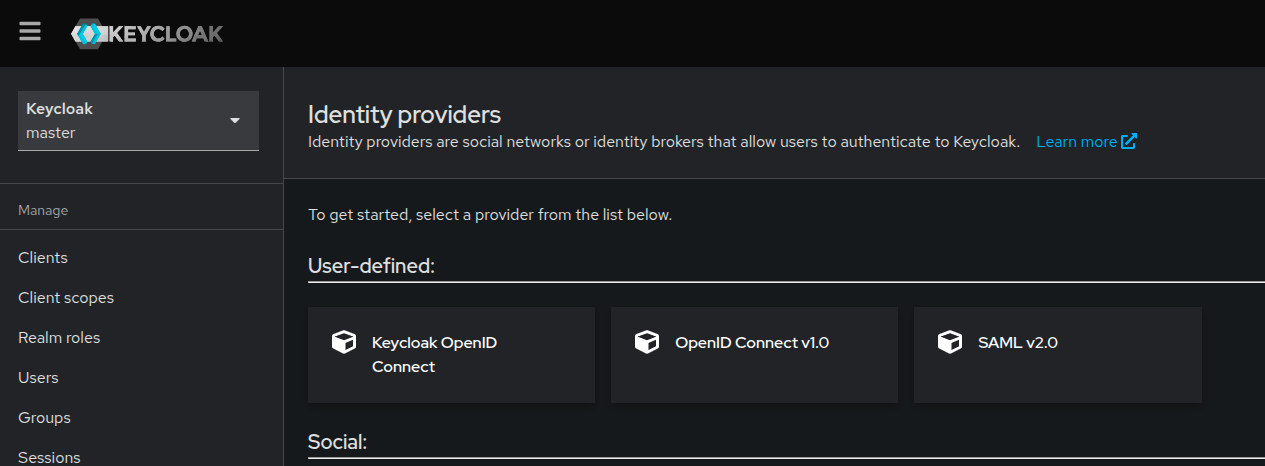
\includegraphics[width=0.9\linewidth]{screenshot007}
		\caption{Protokolle für IdPs in Keycloak}
		\label{fig:screenshot007}
	\end{figure}
	
	\vspace{0.5em}
	\textbf{Grant Typen und Authentifizierungsflüsse:}\\
	Keycloak unterstützt verschiedene \textit{Grant Types}, die beschreiben, wie sich Benutzer oder Clients authentifizieren:
	
	\begin{itemize}
		\item \textbf{Authorization Code Grant:} Benutzer wird zur Keycloak-Loginseite weitergeleitet. Nach erfolgreicher Authentifizierung erhält der Client einen Authorization Code, den er gegen ein Access Token eintauscht. Das Passwort wird dabei nie an die Client-Anwendung weitergegeben.
		\item \textbf{Client Credentials Grant:} Wird für Clients ohne Benutzerinteraktion verwendet. Der Client authentifiziert sich mit seiner Client-ID und einem geheimen Schlüssel (Client Secret), um ein Access Token zu erhalten.
	\end{itemize}
	
	Die \textbf{Client Authentifizierungsmethode} legt fest, wie der Client gegenüber dem Server seine Identität nachweist – z.\,B. mittels Client Secret oder Zertifikat. Während der Grant-Typ die Art der Anmeldung bestimmt, definiert die Client-Authentifizierungsmethode die technische Form des Identitätsnachweises.
	
	Zusätzlich existieren in Keycloak sogenannte \textit{Authentication Flows}, die den Ablauf der Authentifizierung steuern:
	
	\begin{itemize}
		\item \textbf{Standard Flow:} Meist Authorization Code Grant mit Weiterleitung zur Login-Seite.
		\item \textbf{Implicit Flow:} Gibt direkt ein Token zurück, wird aber aus Sicherheitsgründen nicht mehr empfohlen.
		\item \textbf{Direct Access Grant:} Direkte Anmeldung über Benutzername und Passwort, z.\,B. bei Skripten oder mobilen Apps.
		\item \textbf{Device Authorization Grant:} Für Geräte ohne Eingabemöglichkeit, z.\,B. Smart TVs.
		\item \textbf{CIBA (Client-Initiated Backchannel Authentication):} Asynchrone Authentifizierung, z.\,B. über Push-Benachrichtigungen.
	\end{itemize}
	
	\begin{figure}[H]
		\centering
		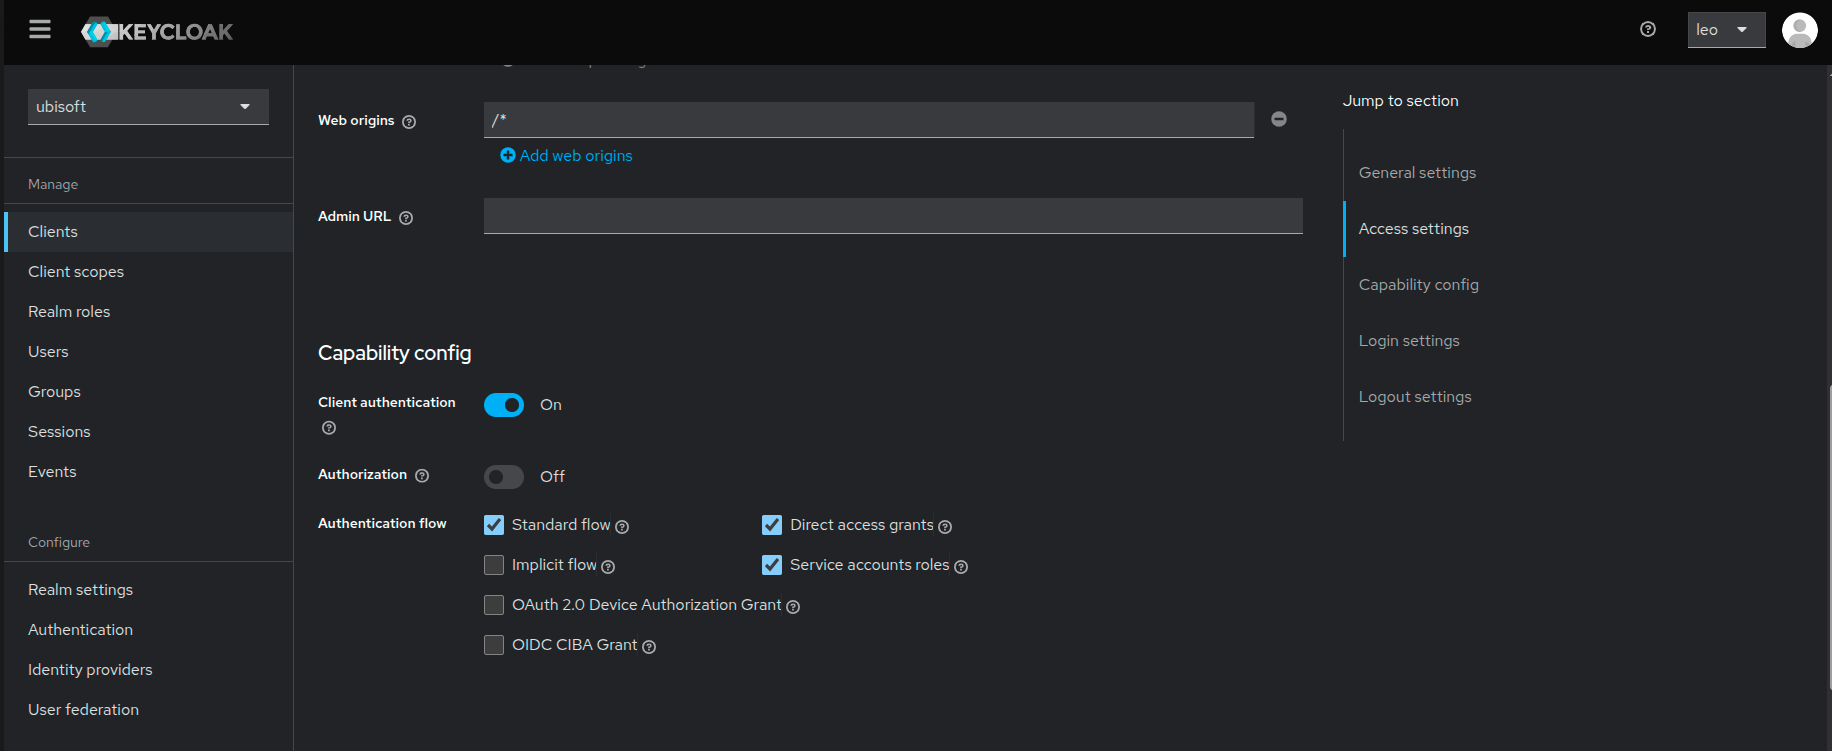
\includegraphics[width=0.9\linewidth]{screenshot013}
		\caption{Beispielhafte Konfiguration von Authentication Flows in Keycloak}
		\label{fig:screenshot013}
	\end{figure}
	
	\vspace{0.5em}
	\textbf{Client-Scope:}\\
	Der \textit{Client-Scope} definiert, welche Benutzerdaten in das Token aufgenommen werden, wenn sich ein Benutzer über einen Client anmeldet. Typische Informationen sind Name, Nachname und E-Mail. Diese Daten werden verschlüsselt übertragen, jedoch besteht ein gewisses Risiko bei Missbrauch oder Diebstahl des Tokens.
	
	\vspace{0.5em}
	\textbf{Rollenmodell:}\\
	Keycloak unterscheidet zwei zentrale Rollentypen:
	
	\begin{itemize}
		\item \textbf{Realm-Rollen:} Gelten global innerhalb eines Realms. Sie eignen sich für übergreifende Rechte, z.\,B. „admin“ für alle Clients.
		\item \textbf{Client-Rollen:} Spezifisch für einen einzelnen Client. Sie erlauben feinere Zugriffskontrolle innerhalb der jeweiligen Anwendung.
	\end{itemize}
	
	\vspace{0.5em}
	\textbf{Service Account Roles:}\\
	Clients können sich in Keycloak auch selbst authentifizieren – ohne Benutzerinteraktion. Wird die \textit{Service Account}-Funktion für einen Client aktiviert, erhält dieser ein eigenes Servicekonto. Dieses Konto kann mit Rollen ausgestattet werden, um Rechte auf bestimmte Ressourcen oder Operationen zu erhalten – z.\,B. für automatisierte Backend-Operationen.
	
	\subsection{Komponenten der Log-Erzeugung}
	Keycloak generiert Logs über eine Kombination aus verschiedenen Frameworks und Komponenten. Grundlage bildet das Logging-Framework von JBoss, wobei moderne Versionen von Keycloak zusätzlich auf das Quarkus-Framework setzen.
	\vspace{0.5em}
	\textbf{Von WildFly zu Quarkus – Technologiewechsel:}\\
	Ursprünglich basierte Keycloak auf dem \textbf{WildFly}-Anwendungsserver\footnote{\url{https://www.wildfly.org/}}, der wiederum die \textbf{JBoss Logging}-Infrastruktur verwendet. Ab Keycloak Version 17 wurde WildFly durch das \textbf{Quarkus}-Framework ersetzt – ein modernes Java-Framework, das speziell für containerisierte und cloud-native Anwendungen entwickelt wurde. Quarkus unterstützt ebenfalls JBoss Logging, sodass bestehende Logging-Mechanismen weiterhin funktionieren.
	
	\begin{figure}[H]
		\centering
		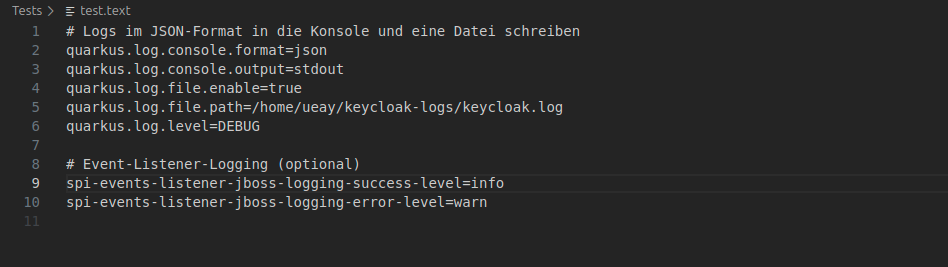
\includegraphics[width=0.9\linewidth]{screenshot008}
		\caption{Beispiel: Aktivierung von Quarkus-Logging in der Keycloak-Konfiguration}
		\label{fig:screenshot008}
	\end{figure}
	
	\vspace{0.5em}
	\textbf{Rolle von JBoss Logging:}\\
	JBoss Logging dient in Keycloak als zentrale Logging-API. Es abstrahiert verschiedene Logging-Backends (wie \texttt{log4j}, \texttt{JUL}, \texttt{Slf4j}) und ermöglicht die strukturierte Ausgabe sicherheitsrelevanter Informationen – z.\,B.:
	\begin{itemize}
		\item \texttt{Realm-ID}
		\item \texttt{Benutzer-ID}
		\item \texttt{IP-Adresse}
		\item \texttt{Event-Typ}
	\end{itemize}
	
	Der Vorteil liegt in der Flexibilität: Entwickler müssen sich nicht auf ein spezifisches Logging-Backend festlegen, sondern können über die einheitliche JBoss-API verschiedene Ausgabekanäle konfigurieren (Konsole, Datei, syslog etc.).
	
	\vspace{0.5em}
	\textbf{Warum nicht Log4j, Logback oder JUL?}\\
	Obwohl es im Java-Ökosystem viele Logging-Frameworks gibt, verzichtet Keycloak bewusst auf deren direkte Verwendung:
	\begin{itemize}
		\item \textbf{Log4j / Logback:} Mächtig, aber externe Abhängigkeiten und teils Sicherheitsrisiken (z.\,B. Log4Shell).
		\item \textbf{JUL (java.util.logging):} Eingebaut, aber funktional begrenzt.
		\item \textbf{Slf4j:} Nur eine Fassade – erfordert Backend wie Logback oder Log4j.
		\item \textbf{System.out / System.err:} Nicht strukturiert, ungeeignet für produktive Logs.
	\end{itemize}
	
	\begin{figure}[H]
		\centering
		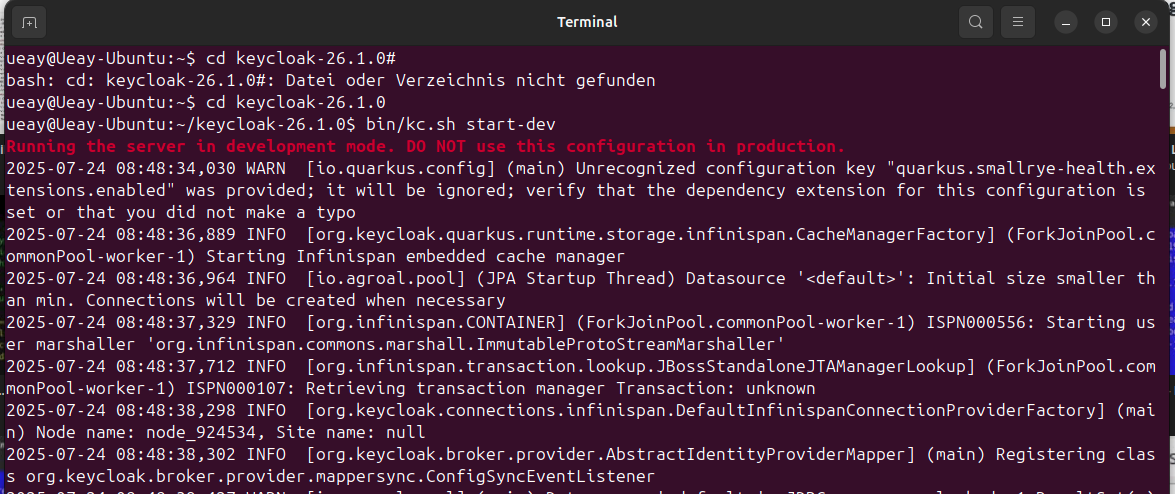
\includegraphics[width=1.1\linewidth]{screenshot014}
		\caption{Log-Ausgaben, wie sie in einer Quarkus-basierten Keycloak-Instanz erzeugt werden}
		\label{fig:screenshot014}
	\end{figure}
	
	\vspace{0.5em}
	\textbf{Vorteile der aktuellen Logging-Architektur:}
	\begin{itemize}
		\item \textbf{Nahtlose Integration:} JBoss Logging ist direkt in Quarkus und die Keycloak-Architektur eingebettet.
		\item \textbf{Sicherheitskontext:} Strukturierte Logs enthalten kontextuelle Daten, die für Auditing und Sicherheitsanalysen wichtig sind.
		\item \textbf{Zentrale Konfiguration:} Log-Level, Ausgabeformate und Ziele können zentral über Konfigurationsdateien gesteuert werden.
		\item \textbf{Konsistenz:} Einheitliches Logging-Verhalten über alle Komponenten hinweg.
	\end{itemize}
	
	Insgesamt stellt JBoss Logging in Kombination mit Quarkus eine robuste, flexible und erweiterbare Logging-Lösung dar, die sowohl Sicherheitsanforderungen als auch Betriebsanforderungen gerecht wird.
	Ein weiterer Baustein ist SLF4J (Simple Logging Facade for Java), das vor allem in vielen externen Bibliotheken der Java-Welt als Logging-Fassade genutzt wird. Quarkus unterstützt SLF4J indirekt, indem es mit einem passenden Backend wie logback oder log4j2 kombiniert werden kann. In Keycloak selbst wird SLF4J jedoch nicht direkt verwendet, da stattdessen vollständig auf JBoss Logging gesetzt wird.
	\vspace{0.5em}
	Für erweiterte oder spezielle Logging-Anforderungen lassen sich Frameworks wie Log4j2 oder Logback über Custom Extensions oder SPIs einbinden. Diese sind nicht standardmäßig in Keycloak aktiv, können aber in Eigenentwicklungen verwendet werden – etwa wenn besondere Formatierungen oder externe Integrationen erforderlich sind.
	\vspace{0.5em}
	Einfache Ausgaben über System.out oder System.err kommen in Keycloak kaum zum Einsatz und dienen allenfalls zu Debug-Zwecken in sehr frühen Initialisierungsphasen. Für produktive Umgebungen sind sie ungeeignet, da sie weder strukturiert noch steuerbar sind und nicht in zentrale Log-Management-Systeme integriert werden können.
	\vspace{0.5em}
	Besonders nützlich ist die Möglichkeit, JSON-basiertes Logging in Quarkus zu aktivieren. Dadurch lassen sich strukturierte Logdaten erzeugen, die sich ideal für den Einsatz in zentralisierten Logging-Stacks wie ELK (Elasticsearch, Logstash, Kibana) oder Loki mit Grafana eignen. Die JSON-Ausgabe wird direkt über eine Property aktiviert (quarkus.log.console.json=true).
	\vspace{0.5em}
	Neben dem klassischen System-Logging bietet Keycloak ein eigenes Audit- und Event-Logging-Subsystem, das unabhängig vom allgemeinen Logsystem funktioniert. Mithilfe des EventListener-SPI können verschiedene Ereignisse – etwa Admin-Änderungen oder Benutzeraktionen – gezielt erfasst werden. Die Ausgabe kann dabei in Form einfacher Logs, in Syslog-Formate oder in benutzerdefinierte Kanäle erfolgen.
	\vspace{0.5em}
	Abschließend unterstützt Keycloak die Integration in externe Logging-Systeme durch Syslog oder Remote Logging. So lassen sich Logs über Tools wie Filebeat an zentrale Systeme weiterleiten (z.B. Logstash oder Cloud-Dienste wie AWS CloudWatch, Google Stackdriver oder Azure Monitor) oder Kubernetes. Dies ist insbesondere in containerisierten oder skalierenden Cloud-Umgebungen entscheidend für Monitoring, Fehleranalyse und Sicherheitsüberwachung.
	
	\subsection{Log-Dateien in Keycloak}
	Logging, bzw. Protokollierung ist ein essentieller Bestandteil für die Überwachung von IT-Systemen. Für das IT-Monitoring dienen Logs zur Verhinderung und Detektion von Anomalien, sei es im Netzwerk, in einem IoT-Gerät oder eben in IAM-Tools. 
	\\[0.5em]
	In Keycloak werden verschiedene Log-Arten unterteilt, wobei die Logs für das Netzwerk, die Access Logs u.A. nicht direkt zu Keycloak gehören.
	Kecyloak unterteilt Logs in folgende Kategorien:
	\begin{itemize}
		\item Server-Logs: Betriebsstatus, Fehler, Debugging-Infos
		\item Event-Logs: Benutzer- und Admin-Events (Event-System)
		\item Audit-Logs: Nachvollziehbarkeit von Änderungen (Admin Events)
		\item Access Logs: Zugriffsversuche und HTTP-Statuscodes (HTTP Layer / Reverse Proxy)
		\item Security Logs: Sicherheitsrelevante Ereignisse und Warnungen
		\item Custom Logs: Erweiterungen und Plugins können eigene Logs erzeugen (SPI)
	\end{itemize}
	Die Logs werden dabei von unterschiedlichen Instanzen in Keycloak erzeugt. Die Server-Logs werden  vom Keycloak-Server selbst erzeugt und weisen die Kategorie \textit{org.keycloak.services} auf. Sie werden mit dem Quarkus-Framework erzeugt.
	\\[0.5em]
	Event-Logs und Audit Logs werden vom Event-System in Keycloak erzeugt, der unter der Kategorie \textit{org.keycloak.events} zu erkennen ist.
	\\[0.5em]
	Access Logs werden auf der Anwendungs- und Netzebene erzeugt- hauptsächlich außerhalb Keycloaks und sind gekennzeichnet als \textit{io.quarkus.http}
	\\[0.5em]
	
	\subsection{Event-Logs}
	Analysiert in dieser Arbeit werden die Event-Logs. Grund hierfür ist, dass diese wichtige Features enthalten, welche das Benutzerverhalten beschreiben. Server-Logs beziehen sich zu sehr auf Netzbasierte Logs und andere Logs, wie Audit-Logs sind Unterkategorien von Events-Logs. Da keine SPI verwendet wird und nur die einzelne Keycloak-Instanz untersucht wird, fallen Custom Logs ebenfalls weg als Teil der Trainingsdaten und Security Logs werden nur erzeugt, wenn es die dazu gehörigen Komponenten dazu gibt,welche hier auch nicht angewandt werden.
	\\[0.5em]
	
	Keycloak unterteilt unter Anderem zwei Arten von Events-Logs:
	
	\begin{itemize}
		\item Admin Logs (Audit Logs)
		\item User Logs (Event Logs)
	\end{itemize}
	
	Die Admin Logs enthalten alle Logs bzgl. den Operationen des Admins und die User Logs nur die Logs von Benutzern, die nicht Admin sein.
	
	\subsection{Aufbau der Event-Logs}
	Folgende Features sind stets in den User Event Logs enthalten:
	
	\begin{itemize}
		\item timestamp
		\item log\_level
		\item category
		\item type
		\item ipAddress
		\item realmName
		\item realmId
		\item clientId
		\item userId
	\end{itemize}
	Man erkennt, dass wichtige Attribute, wie bspw. der Standort des Clients fehlen. Dies liegt an datenschutzrechtlichen Gründen, jedoch erschwert dies Anomalien in den Logs zu erkennen, weil diese anhand des Standortes erkannt werden. Dies muss noch als Störfaktor erkannt werden. Anhand des Standortes können somit schon mal keine Anomalien erkannt werden. Timestamp ist einer der wichtigen Attribute, welche zeigen, um welche Zeit der Log erzeugt wurde. Zur Analyse zeitbasierter Daten eignen sich timestamp als aussagekräftige Information für die LSTM-AE-Hybridmodelle.
	\\[0.5em]
	Desweiteren unterteilt Keycloak noch sogenannte Log-Level. Diese zeigen, ob eine bestimmte Operation erfolgreich war oder nicht oder geben andere Informationen bzgl. einer Operation.
	Bekannte Log-Level sind z.B. INFO, FATAL oder ERROR. Alle Arten finden sich in der Dokumentation \footnote{https://www.keycloak.org/server/logging}.
	Das Loglevel (z.B. FATAL, ERROR, INFO) bestimmt die Art des Logs, z.B. ob es zum Debugging dient oder eine Warnung erschient, entweder ein Fehler oder eine Info.
	\\[0.5em]
	"Category" beschreibt hier die Art des Logs. Da in dieser Arbeit mit Keycloak-Logs gearbeitet wird, kommen insbesondere der JBossLogger \footnote{https://docs.jboss.org/process-guide/en/html/logging.html} und die JPA-Komponente \footnote{https://docs.spring.io/spring-data/jpa/reference/index.html} von Keycloak zum Einsatz.
	\\[0.5em]
	Des weiteren von Bedeutung in den Logs haben die Ereignis-Typen:
	Bspw. ist LOGIN ein Ereignis-Typ bei dem der Benutzer sich anmeldet. Dies wird in Keycloak auch regelmäßig dokumentiert. Andere Ereignistypen sind bspw. TOKEN\_REFRESH, bei dem der Benutzer einen neuen Token bekommt. 
	
	\begin{figure}[H]
		\centering
		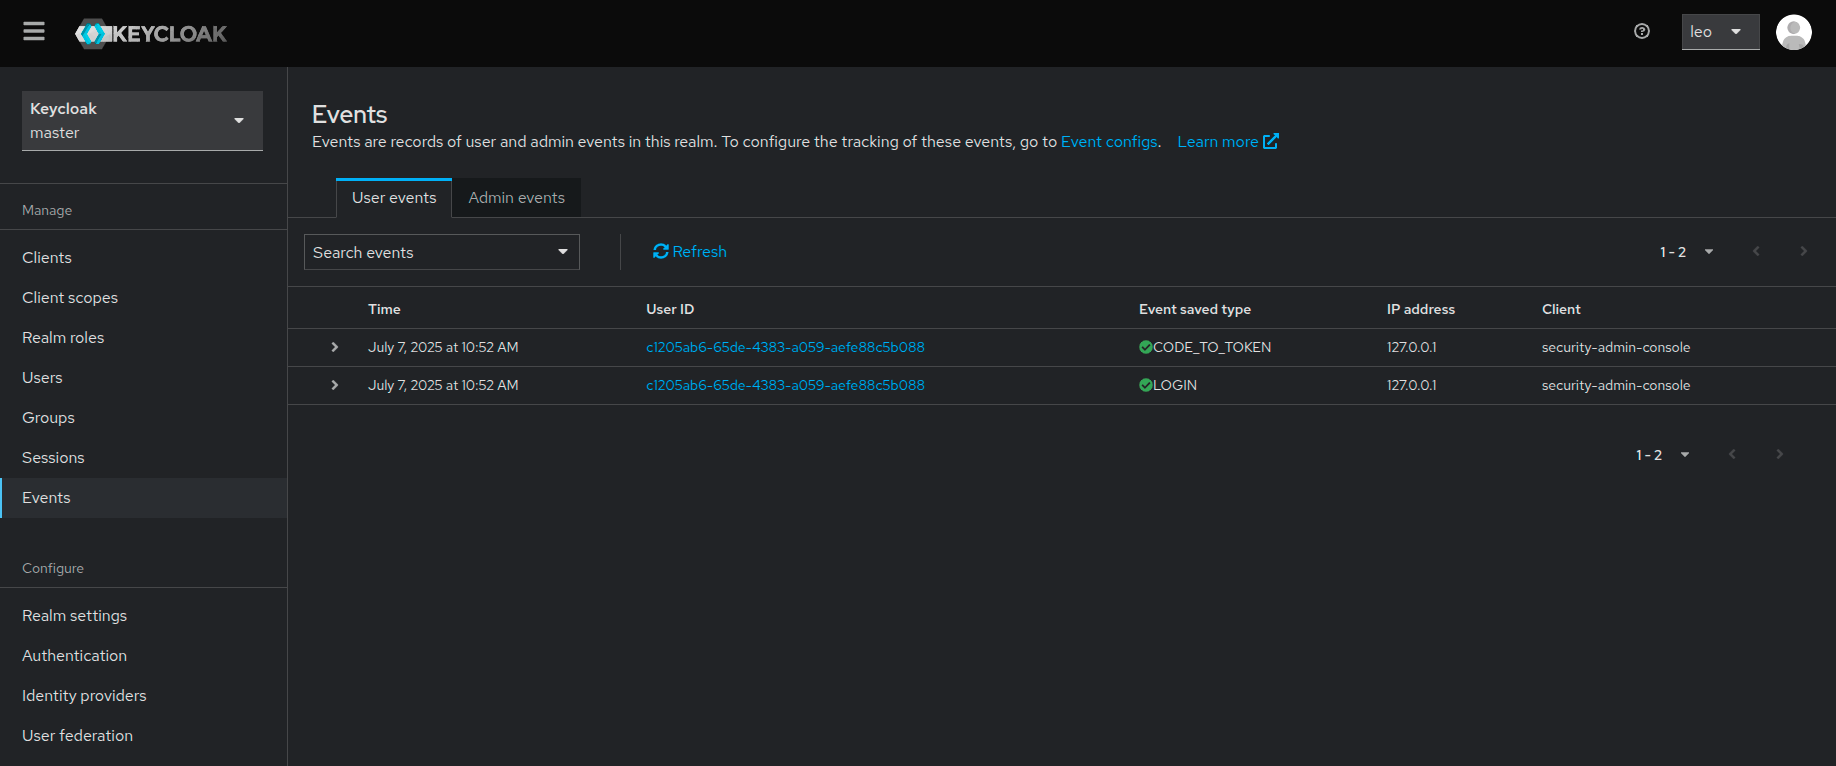
\includegraphics[width=1.0\linewidth]{screenshot002}
		\caption{Beispiel Events nach Eventtyp}
		\label{fig:screenshot002}
	\end{figure}
	
	Je nach Eventtyp werden Features angehängt oder weggelassen, z.B. wird beim Login noch in den Logs die Token-Url, die Art der Verbindung und auch die Art des Authentifizierungsprotokolls angegeben. "Type" steht hier für den Event-Typen. Die wichtigsten Event Type sind dabei folgende:
	
	\begin{itemize}
		\item LOGIN: Log, der generiert wird, wenn sich ein Benutzer erfolgreich einloggt über  Keycloak selbst.
		\item CODE TO TOKEN: Wird erzeugt, sobald der Benutzer sich über seine Anmeldedaten auf dem Keycloak-Server authentifiziert hat und von diesem einen Access Token erhalten hat.
		\item CLIENT LOGIN: Log, der generiert wird, sobald sich der Benutzer über einen Drittanbieter einloggt.
		\item LOGIN ERROR: Fehler beim Login über Keycloak
		\item CODE TO TOKEN ERROR: Anmeldedaten war falsch, Server lehnt Anmeldedaten von Benutzer ab
	\end{itemize}
	In den Admin Logs wiederum sind noch Features enthalten, welche in den normalen User Event Logs nicht vorkommen, u.A. 'operationType': Diese beinhalten typische CRUD-Operationen wie UPDATE, CREATE, DELETE und ACTION \footnote{https://github.com/keycloak/keycloak/blob/main/model/jpa/src/main/java/org/keycloak/events/jpa/JpaAdminEventQuery.java}. 
	\\[0.5em]
	
	\section{Theoretischer Hintergrund der Modelle}
	\subsection{LSTM}
	Long Short-Term Memory (LSTM) ist ein Recurrent Neural Network (\gls{rnn}), welches dazu entwickelt wird zeitabhängige Datenabfolgen zu erkennen und zu analysieren \cite{staudemeyer2019understanding}.
	RNNs sind eine spezielle Klasse von neuronalen Netzwerken, welche dazu entwickelt wurden, sequentielle Daten zu verarbeiten, also Daten bei den die Reihenfolge der zu verarbeitenden Daten entscheiden ist. daher eignen sie sich gut Zeitreihen zu analysieren. RNNs können die nacheinander folgenden, abhängigen Daten anhand eines sogenannten Hidden Errors analysieren: Dabei wird im Hidden Error die zuvor analysierten Daten behalten und mit den nächsten Daten in einem gemeinsamen Kontext verarbeitet. Der Hidden State wird bei jedem Zeitschritt aktualisiert und bildet somit einen gemeinsamen Kontext für die Verarbeitung der aktuellen und vorherigen Eingaben.
	Das Problem an RNNs ist jedoch, dass bei längeren Datensequenzen die Erinnerung der zu weit liegenden Daten verblasst.
	LSTMs gleichen diese Nachteile aus: Sie besitzen über eine Zellstruktur, die gewährleistet, dass auch zu alte Datensequenzen noch erinnert werden.
	Dies wird durch diese drei Bestandteile gewährleistet \cite{hochreiter1997long}:
	\begin{itemize}
		\item \textbf{Forget Gate:} Entscheidet, welche Informationen aus der Zellzustand gelöscht werden sollen.
		\item \textbf{Input Gate:}  Steuert, welche neuen Informationen in den Zellzustand aufgenommen werden.
		\item \textbf{Output Gate:} Bestimmt, welche Informationen aus der Zelle als Ausgabe weitergegeben werden.
	\end{itemize}
	LSTM jedoch haben auch ihre Kapazitäten und auch hier können längere Sequenzen trotz diesen Gates für Verarbeitungsschwierigkeiten sorgen.
	Probleme wie das Vergessen weiter zurückliegender Informationen oder eine ineffiziente Nutzung des Speichers können weiterhin auftreten – wenn auch in deutlich abgeschwächter Form im Vergleich zu Standard-RNNs \cite{hochreiter1997long}.
	LSTM werden in vielen Bereichen, wie z.B: in IoT eingesetzt \cite{wei2022lstm}.
	
	\subsection{Autoencoder}
	Ein Autoencoder ist eine spezielle Form eines neuronalen Netzwerks, das aus zwei Hauptbestandteilen besteht: der Encoder- und der Decoder-Schicht \cite{michelucci2022introduction}.
	\\[0.5em]
	Die Encoder-Schicht komprimiert die Eingabedaten und reduziert ihre Dimensionen auf eine kleinere Repräsentation, die sogenannte Bottleneck-Schicht. Diese Bottleneck-Schicht ist der engste Teil des Netzwerks und zwingt das Modell, die wichtigsten Merkmale der Daten in verdichteter Form zu lernen. Dadurch werden irrelevante oder redundante Informationen herausgefiltert, was den Autoencoder befähigt, die Essenz der Eingabedaten zu erfassen.
	\\[0.5em]
	Die Decoder-Schicht nimmt diese komprimierte Repräsentation und versucht, die ursprünglichen Daten daraus möglichst genau zu rekonstruieren. Das Netzwerk lernt durch Minimierung des Rekonstruktionsfehlers, also der Differenz zwischen Eingabedaten und rekonstruierten Daten. Dieser Fehler ist bedeutend für die spätere Hybridarchitektur.
	\\[0.5em]
	Diese Fähigkeit macht Autoencoder besonders nützlich für Aufgaben wie Anomalieerkennung. Wenn die Rekonstruktion schlecht gelingt (hoher Rekonstruktionsfehler), deutet dies darauf hin, dass die Eingabedaten von den gelernten Mustern abweichen und somit potenziell eine Anomalie darstellen.
	
	\paragraph{Bottleneck und seine Bedeutung}
	Der Bottleneck ist entscheidend, da er die Kapazität des Autoencoders steuert. Ein zu kleiner Bottleneck kann dazu führen, dass wichtige Informationen verloren gehen und die Rekonstruktion schlecht wird. Ein zu großer Bottleneck hingegen erlaubt es dem Netzwerk, einfach die Identität zu lernen und Daten "durchzuschleusen", wodurch der Autoencoder seine Fähigkeit zur Merkmalskompression verliert.
	
	\paragraph{Varianten und Architekturen}
	Neben dem klassischen Autoencoder gibt es weitere Varianten, z.B. den Variational Autoencoder (VAE), der probabilistische Modelle nutzt und generative Fähigkeiten besitzt, oder den Denoising Autoencoder, der lernt, verrauschte Eingaben zu bereinigen. Außerdem können Autoencoder aus mehreren Schichten bestehen (deep Autoencoder), um komplexere Merkmale zu extrahieren.
	
	\paragraph{Vor- und Nachteile}
	Autoencoder bieten den Vorteil, dass sie Merkmale automatisch extrahieren können, ohne dass explizite Labels benötigt werden. Dadurch eignen sie sich gut für unüberwachte Lernaufgaben. Zudem ermöglichen sie eine effiziente Dimensionsreduktion und Datenkompression. Allerdings benötigen Autoencoder zum Trainieren große Datenmengen. Bei einem zu stark eingeschränkten Bottleneck besteht zudem die Gefahr, dass sie eine triviale Identitätsfunktion lernen. Weiterhin ist der Rekonstruktionsfehler nicht immer ein perfekter Indikator für Anomalien, insbesondere bei sehr komplexen Daten. Schließlich kann das Training solcher Modelle rechnerisch sehr aufwendig sein.
	
	\paragraph{Anwendungsbereiche}
	Autoencoder finden Anwendung in der Bildkompression, Anomalieerkennung in Netzwerken oder Produktionsprozessen, Feature Learning vor Klassifikationsaufgaben oder generativer Modellierung.
	
	\begin{figure}[H]
		\centering
		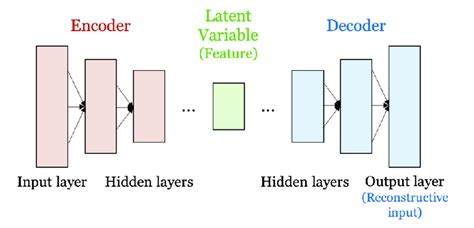
\includegraphics[width=0.7\linewidth]{screenshot004}
		\caption{Visuelle Darstellung der Funktion des AEs, Quelle: https://www.researchgate.net/figure/Structure-of-the-autoencoder\_fig1\_365074431}
		\label{fig:screenshot004}
	\end{figure}
	
	Autoencoder werden für Anomalieerkennung oder auch Dimensionsreduktion verwendet.
	
	\paragraph{Mit dem LSTM kombiniert}
	Autoencoder lassen sich besonders gut mit Long Short-Term Memory (LSTM)-Netzwerken kombinieren, wenn es um sequenzielle oder zeitabhängige Daten geht. Während der klassische Autoencoder oft für statische Daten verwendet wird, können LSTM-Autoencoder zeitliche Abhängigkeiten erfassen und lernen, wie sich Daten über Zeit entwickeln.
	\\[0.5em]
	Ein LSTM-Autoencoder nutzt LSTM-Zellen im Encoder und Decoder, um komplexe zeitliche Muster zu erfassen und zu rekonstruieren. Diese Kombination ist besonders nützlich bei Anomalieerkennung in Zeitreihen, wie etwa in der Überwachung von Maschinenzuständen, Finanzdaten oder Netzwerksicherheit. Anomalien fallen hier oft durch signifikant erhöhte Rekonstruktionsfehler auf, da die zeitlichen Muster nicht gut rekonstruiert werden können.
	\\[0.5em]
	Durch die Fähigkeit von LSTM, langfristige Abhängigkeiten zu modellieren, und die Komprimierung des Autoencoders entsteht ein mächtiges Werkzeug für die Analyse und das Verständnis komplexer, sequenzieller Daten.
	
	\subsection{Isolation Forest}
	Isolation Forest ist ein unüberwachter Lernalgorithmus, welcher durch Partitionen Daten voneinander trennen kann, indem er binäre Bäume erzeugt. Er unterteilt die Daten so lange, bis keine Isolierung der Daten mehr möglich ist. Durch dieses Vorgehen lasen sich auch Anomalien erkennen: Die Anomalien werden je danach erkannt, wie isoliert die Daten eingeteilt wurden. Je isolierter die Datenpunkte aufgeteilt wurden, desto wahrscheinlicher ist es, dass es eine Anomalie ist. Wenn sich Datenpunkte in ihrer Form ähneln, so würde der Algorithmus diese nicht zu stark isolieren. Lassen sich diese jedoch stark anhand ihrer Merkmale isolieren, so  ist es wahrscheinlicher, dass diese keiner üblichen Menge eingeteilt werden kann \cite{liu2008isolation}.
	\\[0.5em]
	\begin{figure}
		\centering
		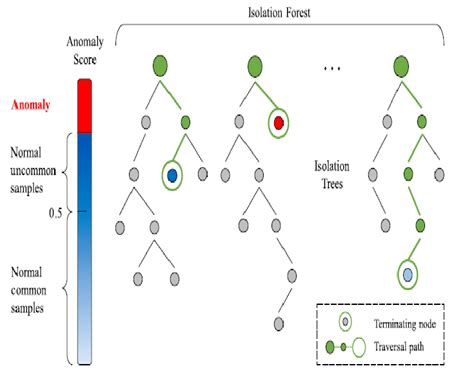
\includegraphics[width=0.7\linewidth]{screenshot005}
		\caption{Visuelle Darstellung der Funktion des AEs, Quelle: https://www.researchgate.net/figure/Anomaly-Detection-using-Isolation-Forest-18\_fig3\_350551253}
		\label{fig:screenshot005}
	\end{figure}
	
	Der Algorithmus erzeugt Isolation Trees, welche aus Blattknoten oder aus einem inneren Knoten besteht,d er eine Testregel enthält, die die Daten in zwei Gruppen aufteilt. Die Testregel besteht aus einem Wert aus der Auswahl eines Merkmals  q und einem Schwellenwert p, so dass alle Datenpunkte, deren Wert für q kleiner als p ist, in den linken Kindknoten kommen, und alle anderen in den rechten Kindknoten.
	\\[0.5em]
	Zum Aufbau eines solchen Baums nimmt man eine Stichprobe von Datenpunkten und teilt sie rekursiv auf, indem man zufällig ein Merkmal und einen Split-Wert auswählt. Dieser Prozess wird so lange wiederholt, bis
	eine maximale Baumhöhe erreicht ist, nur noch ein Datenpunkt übrig ist, oder
	alle Datenpunkte im aktuellen Teilbaum identisch sind \cite{liu2008isolation}.
	\\[0.5em]
	Das Ergebnis ist ein vollständiger binärer Baum, bei dem jeder Datenpunkt in einem Blattknoten isoliert wird.
	\\[0.5em]
	Wenn alle Datenpunkte unterschiedlich sind, dann gilt:
	\begin{itemize}
	\item Es gibt genauso viele Blätter wie Datenpunkte (n).
	
	\item Die Anzahl der inneren Knoten ist n - 1.
	
	\item Insgesamt hat der Baum 2n - 1 Knoten.
	
	\item Der Speicherbedarf wächst also linear mit der Anzahl der Datenpunkte.
	\end{itemize}
	
	Isolation Forest unterteilt jedoch zufällig die Datenpunkte, wobei man die Sinnhaftigkeit des Algorithmus hinterfragen kann.
	
	\subsection{One-Class SVM}
	Mit dem rasanten Wachstum des Internets ist die Sicherheit von Informationssystemen zu einem global wichtigen Thema geworden. Effektive Methoden zur Erkennung von Eindringversuchen sind daher dringend erforderlich. Da viele Angriffe durch die Analyse von System-Logdaten erkennbar sind, wurde ein Ansatz entwickelt, der auf One-Class Support Vector Machines (OC-SVM) basiert und mit abstrahierten Benutzeraudit-Logs aus dem DARPA-Datensatz von 1999 trainiert wurde \cite{li2003improving}. Die Methode nutzt eine nichtlineare Abbildung der Daten in einen höherdimensionalen Raum, um auch nichtlinear trennbare Daten linear trennbar zu machen:
	„Bei nichtlinear trennbaren Daten können wir sie durch eine nichtlineare Abbildung in einen hochdimensionalen Raum transformieren, so dass die Datenpunkte linear trennbar sind.“
	\\[0.5em]
	\begin{figure}
		\centering
		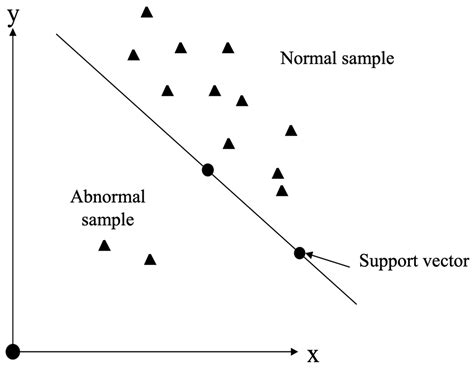
\includegraphics[width=0.7\linewidth]{screenshot006}
		\caption{Visuelle Darstellung  OCSVM. Quelle: https://www.mdpi.com/2076-3417/13/3/1734}
		\label{fig:screenshot006}
	\end{figure}
	Ein zentrales Problem bei One-Class Support Vector Machines (\gls{ocsvm}) besteht darin, dass der Ursprung im Merkmalsraum als Repräsentant für Anomalien dient, obwohl dies in der Realität nicht immer zutrifft \cite{bounsiar2025oneclass}. In ihrer Arbeit erklären die Autoren, dass die Trennung der Zielklasse vom Ursprung (also von den Ausreißern) häufig missverstanden wird. Sie schlagen eine geometrische Interpretation vor, bei der die Zielklasse vom übrigen Raum getrennt wird, insbesondere wenn ein Gauß-Kernel verwendet wird.
	
	\subsection{DBSCAN}
	DBSCAN ist ein dichtebasiertes Cluteringverfahren, dass Datenpunkte anhand ihrer Dichte zu anderen Punkten klassifizieren kann.
	Die Dichte wird durch die Anzahl der Nachbarpunkte innerhalb eines Radius (Eps) gemessen, wobei mindestens eine Mindestanzahl von Punkten (MinPts) in diesem Radius vorhanden sein muss \cite{ester1996dbscan}. Die Wahl dieser Parameter ist entscheidend für den Erfolg der Klassifizierung.
	
	\begin{figure}[H]
		\centering
		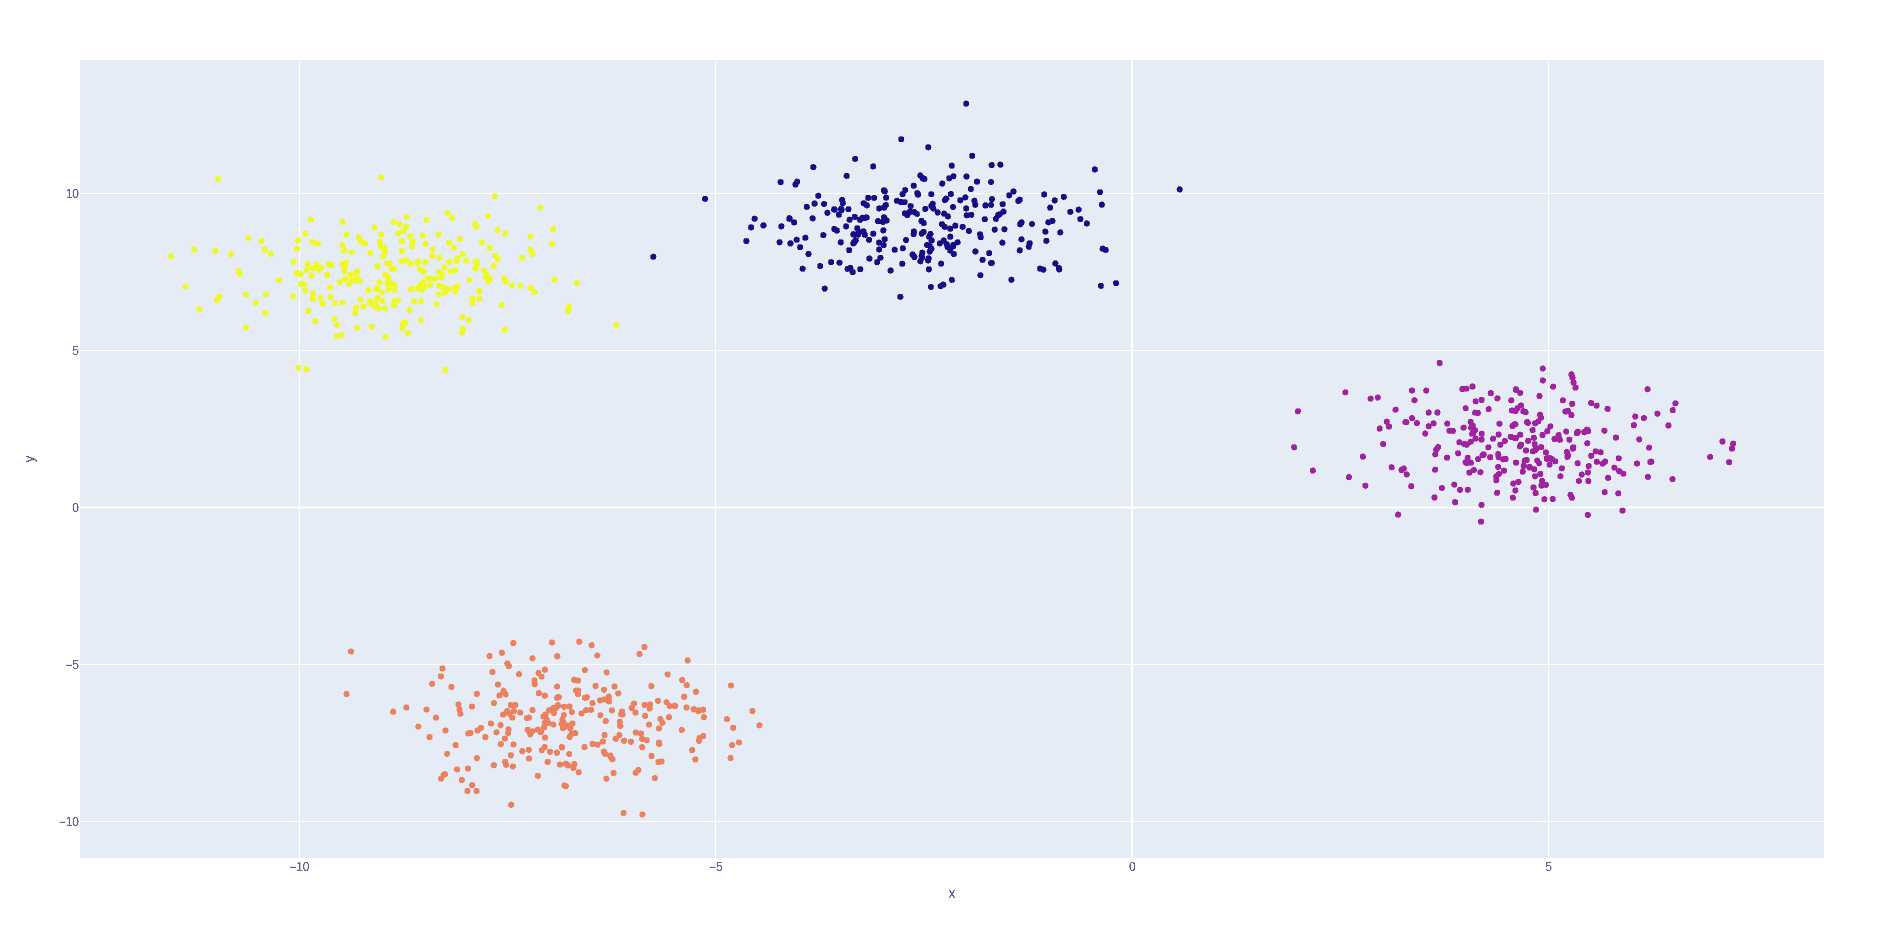
\includegraphics[width=0.9\linewidth]{screenshot015}
		\caption{Beispiel DBSCAN-Cluster, Quelle: \url{https://www.baeldung.com/wp-content/uploads/sites/4/2023/04/clusters.png}}
		\label{fig:screenshot015}
	\end{figure}
	
	Der Algorithmus läuft folgendermaßen ab:
	Man startet von einem bestimmten Punkt p. Daraufhin werden alle Punkte gesucht, welche sich in der Nähe von p befinden. Sobald eine Mindestanzahl von Eps erreicht ist, die auch durch MinPts festgelegt wird, so bildet sich ein Cluster. Danach werden alle Punkte die nun zu einem Cluster gehören, aus einer Liste an verbleibenden Punkten herausgenommen. Daraufhin wird p zufällig an einen weiteren Ort im Raum platziert, wo noch kein Cluster gebildet wurde. Dies geschieht solange, bis keine Punkte in der Liste übrig sind. Die restlichen Punkte, die keinem Cluster zugeordnet sind, heißen Noises. Wenn es zu viele Noises gibt, heisst das, dass nicht effizient klassifiziert wurde \cite{ester1996dbscan}. 
	
	\subsection{Alternative Algorithmen}
	Wie bereits im Forschungsstand erwähnt, wurde als Alternative zu DBSCAN auch das hierarchische Verfahren HDBSCAN (Hierarchical Density-Based Spatial Clustering of Applications with Noise) in Betracht gezogen. HDBSCAN ist in vielerlei Hinsicht robuster als DBSCAN, insbesondere bei der Identifikation von Clustern in hochdimensionalen oder verrauschten Daten. Ein Vorteil von HDBSCAN ist, dass es keine globale Dichte-Schwelle benötigt und sich besser an lokale Datenstrukturen anpasst. Aufgrund der derzeit noch begrenzten Anzahl an Studien und praktischen Erfahrungswerten zu HDBSCAN im konkreten Anwendungsbereich wurde jedoch auf den Einsatz verzichtet. Für zukünftige Arbeiten wäre es durchaus interessant, HDBSCAN in Kombination mit LSTM-Autoencodern (LSTM-AE) näher zu untersuchen.
	\\[0.5em]
	Darüber hinaus wurden auch weitere Anomalieerkennungsverfahren wie K-Means und LOF (Local Outlier Factor) evaluiert. Beide Methoden sind grundsätzlich für die Anomalieerkennung geeignet, insbesondere bei kleineren und klar strukturierten Datensätzen. Allerdings stoßen K-Means und LOF bei großen, komplexen oder verrauschten Datenmengen an ihre Grenzen. K-Means ist dabei empfindlich gegenüber Ausreißern und erfordert die Festlegung der Clusteranzahl vorab. LOF erkennt Ausreißer, indem es die lokale Dichte eines Datenpunkts mit der seiner Nachbarn vergleicht und Punkte mit stark abweichender Dichte als potenzielle Anomalien markiert. Allerdings wird LOF mit zunehmender Datenmenge zunehmend ineffizient.
	
	\section{Implementierung}
	\subsection{Hybridmodelle mit LSTM-AE}
	Generell wurden die Modelle nach der selben Architektur gebaut:
	
	\begin{figure}[H]
		\centering
		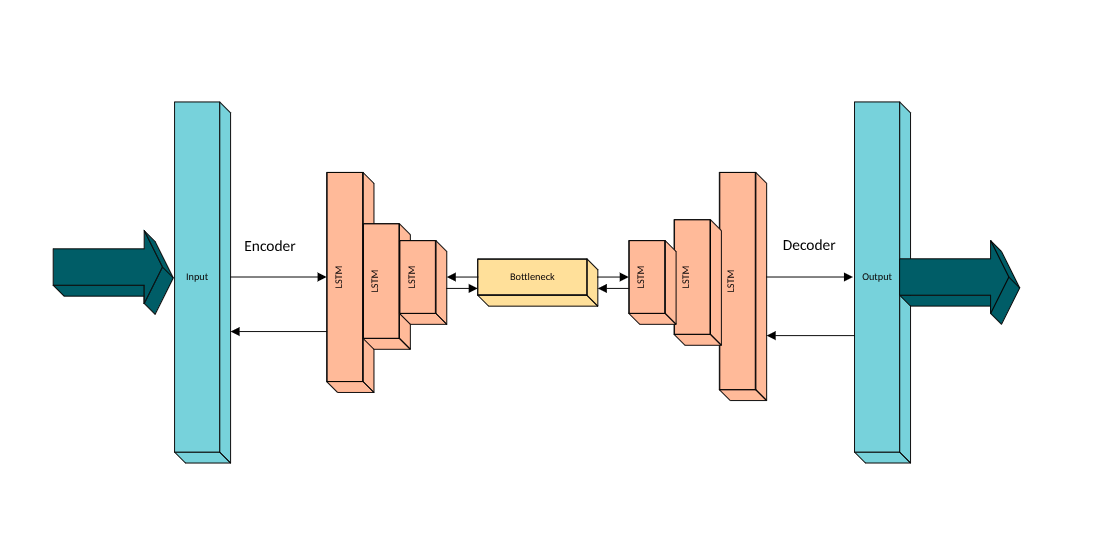
\includegraphics[width=0.7\linewidth]{screenshot001}
		\caption{Architektur}
		\label{fig:screenshot001}
	\end{figure}
	
	Die Daten werden zuerst in kategorische oder numerische Daten aufgeteilt. Absichtlich werden NaN-Werte und unklare Werte nicht bereinigt, sondern in eine eigene Kategorie gefasst. Dies ist wichtig, da auch solche Werte Anomalien darstellen und die Bereinigung dieser Daten dafür sorgen würde, dass potenzielle Gefahrquellen unerkannt bleiben. NaN-Werte können außerdem bspw. bei falschen Accounts oder vielleicht bei Bots auftreten, weshalb es wichtig ist, diese in der Analyse beizubehalten. Zudem ist der LSTM-AE sehr gut darin verschieden Daten, sei es kategorisch oder numerisch zu erkennen, weshalb solch eine Vorverarbeitungsweise gewählt wurde.
	\\[0.5em]
	Die Logs werden separat je nach Training, Test und Validierung in Dateien gepackt und dann zu Beginn ausgelesen. Zuerst werden diese Daten vorverarbeitet. Die Features werden danach automatisch in numerische, kategorische oder nicht definierte Daten eingeteilt.Die eingeteilten und bereinigten Daten werden danach wieder zusammengefügt. Alle drei Dateien, also Evaluierungs-, Test- und Trainingsdateien werden dabei einzeln bereinigt und zusammengefügt. Darauf hin werden alle Daten mit der standardisiert und skaliert. Da der LSTM-AE nur mit sequentiellen Daten arbeiten kann, wurden diese Dateien in Sequenzen aufgeteilt.
	\\[0.5em]
	Es wurden folgende Parameter bestimmt:
	
	\begin{table}[h]
		\centering
		\begin{tabular}{ll}
			\toprule
			\textbf{Parameter}       & \textbf{Wert}            \\
			\midrule
			seq\_length             & 15                       \\
			batch\_size             & 128                      \\
			encoder\_layers         & [256, 128, 64]         \\
			decoder\_layers         & [64, 128, 256]         \\
			dropout\_rate           & 0.2                      \\
			learning\_rate          & 0.0001                   \\
			\bottomrule
		\end{tabular}
		\caption{Bestimmte Parameter der Modellkonfiguration}
		\label{tab:model_params}
	\end{table}
	
	Die Trainingsfehler, bzw. Rekonstruktionsfehler, also die Daten, welche nicht klar klassifiziert werden konnten, werden danach jeweils mit einem der vorimplementierten Modelle trainiert. Dies ist auch eine Vorangehensweise, welche schon angewandt wurde \cite{malhotra2016lstm}.
	Die Implementierung erfolgt in Form einer modularen Pipeline. Zunächst wird der LSTM-Autoencoder sequenziell trainiert und die Rekonstruktionsfehler für die Daten berechnet. Anschließend werden diese Fehler unabhängig voneinander als Eingabe für die verschiedenen Anomalieerkennungsmodelle (Isolation Forest, One-Class SVM, DBSCAN) verwendet. Dadurch kann jedes Modell separat trainiert, getestet und evaluiert werden, was eine modulare Struktur gewährleistet, auch wenn die gesamte Umsetzung in einem Jupyter Notebook erfolgt.
	
	\subsubsection{Implementierung: Isolation Forest}
	Die Trainingsfehler, also die Daten, welche nicht klar klassifiziert werden konnten, werden danach jeweils mit einem der vorimplementierten Modelle trainiert. Im Fall des Isolation Forest wird ein auf Entscheidungsbäumen basierender Algorithmus genutzt, der speziell für die Erkennung von Ausreißern in hochdimensionalen Daten entwickelt wurde. Dabei wird das Modell auf den Fehlerwerten der Trainingsdaten fitten, um anschließend auf die Testdaten angewendet zu werden. Die Vorhersage klassifiziert dabei jeden Datenpunkt als normal (1) oder anomal (-1). Diese Ergebnisse werden binär kodiert, um eine einfache Auswertung zu ermöglichen. Da die zugrunde liegenden Daten sequenzbasiert aufgebaut sind – beispielsweise aus Zeitreihen bestehen – wird zusätzlich ein Abgleich mit den tatsächlichen Labeln vorgenommen. Hierzu wird aus den Zielwerten der Testdaten die letzte Klasse jeder Sequenz extrahiert, um sie mit den Vorhersagen vergleichen zu können.
	
	\subsubsection{Implementierung: OCSVM}
	Für die Umsetzung der One-Class SVM wird das Modell mit einem sehr niedrigen nu-Wert von 0.005 initialisiert. Dieser Wert steuert die erwartete Rate an Ausreißern im Trainingsdatensatz. Zusätzlich wird der Parameter gamma auf 50 gesetzt, was die Einflussweite einzelner Datenpunkte auf die Entscheidungsgrenze definiert. Anschließend wird das Modell mit den Fehlerwerten der Trainingsdaten trainiert, die zuvor durch ein Rekonstruktionsmodell (z.\,B. LSTM-Autoencoder) erzeugt wurden.Nach dem Training wird die One-Class SVM auf die Fehler der Testdaten angewendet. Die Methode predict() liefert Vorhersagen in Form von 1 (normal) oder -1 (anomal). Diese Vorhersagen werden daraufhin in binäre Werte (1 = Anomalie, 0 = normal) umgewandelt. Um die Klassifikation korrekt auszuwerten, wird wie auch bei den anderen Verfahren für jedes Sequenzfenster das zugehörige Label aus den ursprünglichen Testlabels extrahiert. Daraus entsteht ein Label-Vektor, der mit den Vorhersagen verglichen wird.
	
	\subsubsection{Implementierung: DBSCAN}
	Im Fall von DBSCAN handelt es sich um ein dichtebasiertes Clusteringverfahren, das keine explizite Trainingsphase benötigt. Das Modell wird direkt auf die Fehlerwerte der Testdaten angewendet. Als Parameter wird eps = 0.05 gewählt, um die maximale Nachbarschaftsdistanz für die Punkte zu begrenzen, sowie min\_samples = 40, was die Mindestanzahl an Nachbarn definiert, um als Kernpunkt eines Clusters zu gelten. Die Methode fit\_predict() gibt für jeden Punkt entweder eine Clusterzuweisung (0, 1, …) oder -1 zurück – letzteres kennzeichnet Datenpunkte, die als Rauschen bzw. Anomalien erkannt wurden.
	Analog zu den anderen Verfahren werden die -1-Werte in binäre Anomalien umgewandelt. Die tatsächlichen Labels werden erneut sequenzbasiert aus dem vollständigen Label-Vektor extrahiert. Abschließend wird ein Classification Report erzeugt, um die Qualität der durch DBSCAN erkannten Anomalien gegenüber den echten Anomalien zu evaluieren.
	
	\subsection{Alternative Architekturen}
	Es bestand die Möglichkeit, vorher eines der Algorithmen zu trainieren und danach die selben Daten nochmals in den LSTM-AE. Es ist also der umgekehrte Weg, welcher auch in einer Masterabeit verwendet wurde, bei dem ein Hybridmodell zwischen IF und LSTM-AE erstellt wurde \cite{hybrid_if_lstm2023}.
	Desweiteren gibt es auch Architekturen, welche nur DBSCAN und OCSVM benutzen, wobei die Daten zuerst von OCSVM verwendet werden und später durch DBSCAN geclusert werden \cite{pu2021hybrid}.
	\\[0.5em]
	Es gab auch Ideen, für größerer Hybridmodelle. U.A. wurde eine große Kombination aus LSTM-AE, DBSCAN und IF erstellt. Die Daten werden demnach zuerst vom LSTM-AE verarbeitet. Die Fehler daraus werden geclustert durch DBSCAN, falls es auch unterschiedliche Fehlerarten gibt. schlussendlich entschiedet IF, welche Anormal sind und welche nicht.
	\\[0.5em]
	Diese Alternativen wurden jedoch nicht umgesetzt, da sie zu komplex sind, insbesondere, weil in dieser Arbeit nur verhaltensbasierte Anomalien verarbeitet werden, welche sich in Event-Logs zeigen. Solch ein komplexes Modell wurde auch erwogen, weil zu Beginn diskutiert wurde, Modelle in Cloud-Umgebungen zu verwenden, weshalb ein robustes Modell notwendig ist, um große Datenmengen effizient zu verarbeiten und daraus Anomalien zu erkennen. Schlussendlich entschied man sich jedoch für eine Kombination aus LSTM-Autoencoder und jeweils einem klassischen Algorithmus, da so der Vergleich der einzelnen Verfahren deutlich klarer und nachvollziehbarer bleibt.
	\\[0.5em]
	Darüber hinaus ermöglichen einfachere hybride Modelle eine bessere Interpretierbarkeit und Wartbarkeit, was in produktiven Systemen von großer Bedeutung ist. Komplexe Modelle bringen häufig einen erheblichen Mehraufwand bei der Parametrisierung und dem Training mit sich, der in Bezug auf den Erkenntnisgewinn und die praktische Anwendung nicht immer gerechtfertigt ist.
	\\[0.5em]
	Zudem ist zu beachten, dass verhaltensbasierte Anomalien in Event-Logs oftmals durch zeitliche Muster und Sequenzen charakterisiert sind, was der LSTM-Autoencoder durch seine Fähigkeit zur Modellierung von Zeitreihen besonders gut abdeckt. Die ergänzenden klassischen Algorithmen dienen hier vor allem zur Unterstützung bei der Erkennung von Ausreißern oder Clustern, wodurch eine effiziente und dennoch aussagekräftige Erkennung gewährleistet wird.
	\\[0.5em]
	Durch die klare Trennung der Methoden in der gewählten Architektur lassen sich zudem die jeweiligen Stärken und Schwächen besser analysieren und bewerten, was den wissenschaftlichen Vergleich und die spätere Optimierung erleichtert.
	
	
	\section{Möglichkeit 1: Generierung der Logs}
	\subsection{Angriffsfälle}
	Nach jetzigem Stand gehören zu den häufigsten Insider-Attacken in IT-Systemen u.A. der Missbrauch von hohen Privilegien, Rollen und Recht, Datendiebstahl, sowie der Manipulation wichtiger Daten, wie bspw. dem Löschen von wichtigen Dateien \cite{singh2022insiderthreats}. Brute-Force Angriffe gehören ebenfalls zu den wichtigsten Attacken. Es wurden jene Angriffsmöglichkeiten umgesetzt, welcher auch am wahrscheinlichsten auftreten und auch in den Logs erkennbar sind. Datendiebstahl bspw. lässt sich nicht direkt erkennen in Keycloak, weil in den Log-Dateien wenig zum Upload großer Dateien etwas angegeben wird. Es wird erwartet, dass Angriffe, wie dem Stehlen von Rollen in Keycloak eher auftreten würden, sowie Brute-Force Attacken, weshalb diese Anwendungsfälle umgesetzt werden. Sie sind zudem in den Logs bspw., durch Attribute wie dem Event Typ LOGIN\_ERROR erkennbar. 
	\\[0.5em]
	Da der Fokus dieser Arbeit auf dem Gebiet des anomalen Benutzerverhaltens liegt, werden bewusst Angriffsfälle wie DDoS-Attacken nicht berücksichtigt. Von daher werden nur folgende Angriffsfälle modelliert in den Logs:
	
	\begin{itemize}
		\item \textit{Anwendungsfall 1: }Brute-Force Attacken bei der Anmeldung
		\item \textit{Anwendungsfall 2: } Löschen und Änderungen an wichtigen Clients, Usern, Passwörtern und Realms
		\item \textit{Anwendungsfall 3: } Erlangung wichtiger Rollen des Admins, wie bspw. manage-users, und realm-admin
		\item \textit{Anwendungsfall 4: } Häufiges Abfragen derselben Quelle
	\end{itemize}
	Zudem werden bekannte Anomalien wie ungewöhnlichen IP-Adressen und ungewöhnliche Anmeldezeitpunkten bei der Generierung berücksichtigt. Es wird darauf geachtet, hohe Variabilität bei den Angriffen zu gewährleisten.
	
	\subsection{Automatische Erstellung der Keycloak-Logs}
	Die Logs werden durch ein Python-Skript erzeugt.
		\\[0.5em]
	Der erste Anwendungsfall wurde so umgesetzt, dass eine Abfolge von mehreren Logs erzeugt wird, welche den Event Typen LOGIN\_ERROR enthalten. Die Logs können ungewöhnliche timestamps und/oder IP-Adressen enthalten, was aber nicht immer der Fall sein muss, weil schon die Abfolge dieses Event Types anomal ist. Da in Keycloak generell selbst bestimmt werden kann, ab wie vielen Anmeldeversuchen, die IP-Adresse gesperrt wird, muss bei der Generierung der Logs ein Raum angegeben werden dazu. Es werden dabei ca. zwischen 3 bis mehrere 15 Log-Abfolgen zufällig erzeugt.Der Grund für diese Auswahl besteht aus Erfahrung: Ab 3 fehlgeschlagenen Anmeldeversuchen wird das Verhalten als anomal gedeutet, auch wenn es häufig nicht der Fall ist, ab 15 sollte dann schon es eine Anomalie sein, wie alles darüber. Man entschied sich dabei die Zahl gering zuhalten, damit die Sessions nicht zu lang werden.
	\\[0.5em]
	Für den zweiten Anwendungsfall sind Features, welche auf Updates oder dem Löschen von Entitäten deuten, wie z.B. DELETE, UPDATE\_PASSWORD oder auch UPDATE\_PROFILE. Auch hier wird eine Anzahl an Logs gewählt, welche auf das anomale Verhalten hindeuten. Es werden mindestens 5 Abfolgen erzeugt, welche eines der erwähnten Event Typen beinhaltet. Hierbei wird auf Variabilität geachtet, für mehrere Anwendungsmöglichkeiten, damit keine zu strikte Abfolge erzeugt wird. Denn wenn das Modelle stets das gleiche Angriffsmuster erkennt mit den selben Features, dann kann es zu Overfitting führen und das Modelle kann keine neue Angriffe erkennen. Bspw. werden die Logs so erzeugt, dass die Features unterschiedlich zusammengesetzt werden können. Wenn ein Feature "authType" bspw. mit dem Event Typ UPDATE ständig auftritt, dann ist es wahrscheinlich, dass das Modell stets diesen Zusammenhang nur kennt und keine weiteren.
	\\[0.5em]
	Natürlich ist der Nachteil dieser Art von Log-Generierung dass auch Logs erzeugt werden, welche ein Recht schwaches oder stupides Angriffsmuster haben, welche eher nicht auf einen Angriff,sondern auf zufällige Auswahl von Ereignissen hindeutet, welche keinen Zusammenhang haben. Um das zu verhindern, wurde eine Logik eingebaut, die dafür sorgt, dass die Regeln im System Keycloak nicht widersprüchlich sind. Bspw. darf es einen Benutzer mit eindeutiger ID nur in einem Realm geben und den Admin auch nur einmal in ganz Keycloak. Es wird fest definiert, welche Rollen dem Admin zugeordnet sind und damit eine hohe Priorität haben und welche Rollen auch für normale Benutzer gelten. Es wurde auch darauf geachtet, dass der normale Benutzer keine Features wie dem "operationType" benutzen kann, also alle CRUD-Operationen auf den Entitäten. Dieses Feature sind nur in den Admin-Logs enthalten. Es wurde auch klar definiert, dass ein Benutzer genau einer Session angehört und auch nur einem Realm, es sei denn, es ist ein Angreifer.
	\\[0.5em]
	Der 3. Anwendungsfall prüft, ob es mehrere Admins gibt und ob ein eigentlich normaler Benutzer plötzlich Admin wird. Hier wurde auch bei der Generierung der Logs darauf geachtet, dass die Sessions dabei einen Benutzer wählen, welcher zu Beginn keine Admin-Rollen hat und plötzlich mehrere Admin-Rollen bekommt, bzw. auch selbst die Admin-Id erhält. Die Rollen, die dabei überprüft werden sind bspw. admin, realm-admin und manage-users.
	\\[0.5em]
	Der 4. Anwendungsfall beinhaltet mehrere Logs. welche die Admin-Operation GET stets enthalten auf die gleiche Quelle. Dies kann ein Benutzer oder ein Client sein.
	\\[0.5em]
	Normale User-Sessions enthalten keine anomalen IP-Adressen oder ungewöhnliche timestamps. Ein ungewöhnlicher timestamps in diesem Fall sind die Uhrzeiten zwischen Abend 0 Uhr bis 6 Uhr Morgens. Natürlich ist dies stets Interpretationssache, welche Uhrzeiten normal und welche unnormal sind. Es kann auch Benutzer geben,welche gerne im Homeoffice auch Abend arbeiten und eigentlich damit kein anormales Verhalten zeigen. Jedoch wird hier in dieser Arbeit vom Regelfall ausgegangen, also dass es anormal ist, wenn ein Benutzer Mitternachts eingeloggt ist.
	\\[0.5em]
	Die Bestimmung von unnormalen IP-Adressen wurde überwiegend aus Quellen der IANA\footnote{https://www.iana.org/assignments/iana-ipv4-special-registry/iana-ipv4-special-registry.xhtml} übernommen.
	\\[0.5em]
	\begin{figure}[H]
		\centering
		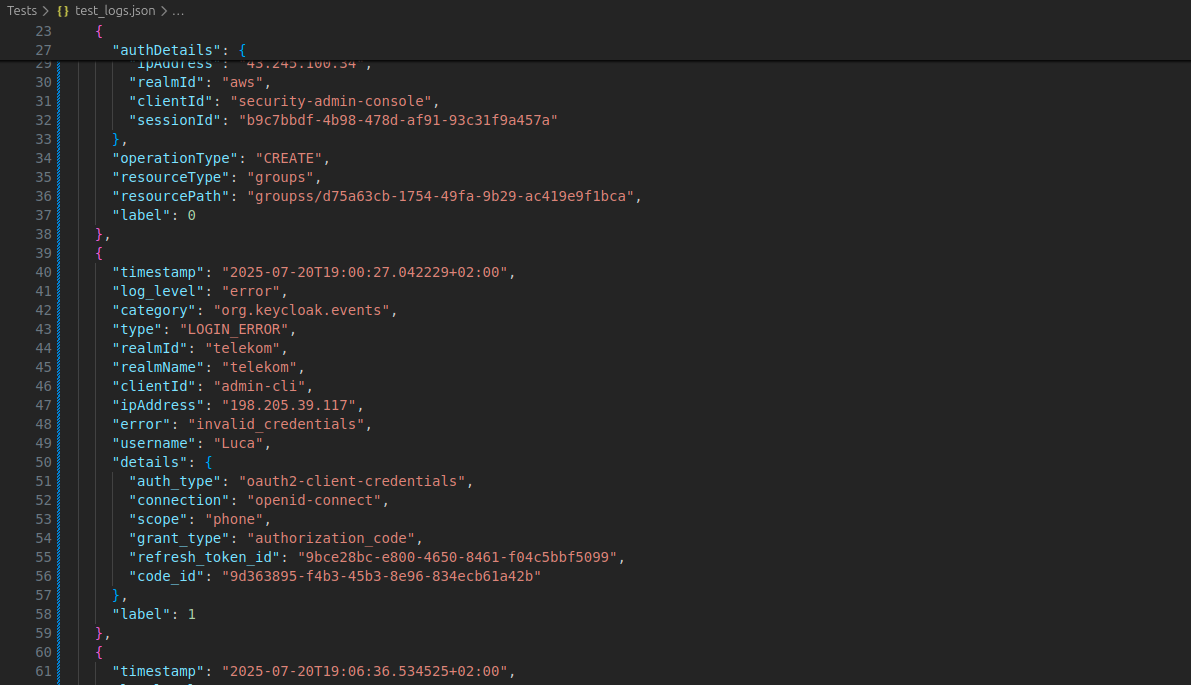
\includegraphics[width=1.0\linewidth]{screenshot009}
		\caption{Ausschnitt der generierten Logs}
		\label{fig:screenshot009}
	\end{figure}
	Bei der Generierung der Log-Daten wurde auch beachtet, dass nicht nur Normale und Anormale Benutzer-Sessions erzeugt werden, sondern auch Sessions, welche sich nicht klar zuordnen lassen. Dies wird dann auch \textit{Noise} genannt. Noise tritt des Öfteren in realen Anwendungsfällen auf, weil auch normale Benutzer manchmal bspw. priorisierte Rollen erhalten müssen aus Management-Gründen oder auch zu oft das Passwort ändern aus eigenen Bedenken der Sicherheit. Die Modelle würden dazu tendieren diese als Anormal zu deuten. Dies wird hier verhindert, indem noch im Script mit Absicht Noises erzeugt werden.
	
	\subsection{Problematik dieser Lösung}
	Bei der Generierung der Logs wurden nur die wichtigsten Features erzeugt, welche auf notwendig, sind um Anomalien zu finden. Im Rahmen der Arbeit war es nicht möglich, detaillierte Informationen über die genaue Anlage und Struktur der Event Typen im Keycloak-System zu erhalten, da hierzu keine umfassende Dokumentation vorlag und der Zugriff auf administrative Ressourcen eingeschränkt war. Daher wurde die Analyse auf die verfügbaren und typischen Log-Daten gestützt, die generische Features und Muster der Systemaktivitäten widerspiegeln. Diese Einschränkung wird im weiteren Verlauf berücksichtigt und limitiert die Tiefe der Auswertung.
	\\[0.5em]
	Eine Herausforderung dieser Arbeit war, die Wahrscheinlichkeit zu bestimmen, wann eine Session Anormal ist, wann normal und wann es einfach Noise, also normale Logdaten,welche aber Anomalien ähneln, ist. Da Anomalien selten sind wurde ein Wert für die Wahrscheinlichkeit des Auftretens einer Anomalie 2 Prozent bestimmt. Da diese Entscheidung auf Intuition basiert, wird nicht gewährleistet, dass die Daten keine realen Daten abbilden können. Dies beeinflusst das Ergebnis.
	\\[0.5em]
	Aufgrund dieser Nachteile und den resultierenden Ergebnissen, wurde dieser Ansatz an den Modellen getestet, wird aber verworfen.
	
	\section{Möglichkeit 2: Datenbeschaffung als Alternative}
	Da die Generierung der Daten eine hohe Aufwendigkeit benötigt, wird stattdessen der sinnvollere Ansatz verwendet, echte Keycloak-Daten zu beschaffen. Jedoch werden es keine Daten aus Unternehmen, da man keine datenschutzrechtlichen Risiken eingehen will. Stattdessen wurde die Idee angenommen, über eine lokale Keycloak-Instanz selbst Log-Daten zu generieren. Da dieser Weg zeitaufwendig ist, wurde in Betracht gezogen, über sogenannte Selenium-Tests Angriffsszenarien zu inszenieren und ebenfalls durch Selenium-Tests gewöhnliche Keycloak-Daten zu generieren. Was dabei als normale Keycloak-Logs zu verstehen ist, wird dadurch  herausgefundenen, sich an firmeninternen Logs zu orientieren.
	
	\subsection{Anbindung der Keycloak-Api}
	Um Zugriff auf die Keycloak-Logs zu erhalten, ist es notwendig, selbst eine Keycloak-Instanz aufzusetzen und selbst als Admin zu navigieren. 
	Um nun an die Logs aus Keycloak, also die die aus Quarkus hauptsächlich aus generiert werden, zu kommen, muss man zuerst die benötigten Ressourcen finden. Standard gemäß benötigt man Admin-Rollen, um an sensible Informationen wie User Event Logs und den Admin Event Logs selbst zu gelangen. Man benötigt zunächst einmal die korrekten Authentifizierungsmittel, damit man auch Rechte erlangt, um auf die Events zugreifen zu dürfen.
	\\[0.5em]
	Der gewählte Grant Typ hierfür ist \textit{Client Credentials}. Hierbei meldet man sich über einen beliebigen Client an. man benötigt noch das Client-Secret und schickt dieses mit den anderen Daten ab.
	\\[0.5em]
	\begin{figure}[H]
		\centering
		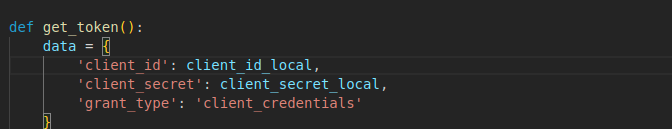
\includegraphics[width=0.9\linewidth]{screenshot010}
		\caption{Daten, die an den Keycloak-Server gesendet werden müssen}
		\label{fig:screenshot010}
	\end{figure}
	Man erhält dadurch den Token, welcher benötigt wird, um nun an die Event Logs zu importieren. Im Token sind die Zugriffsrechte geschildert, die der jeweilige Admin hat, er benötigt die Rollen, die dazu benötigt ist, Benutzer zu verwalten,welche dann auch im Token aufgelistet ist. Nun wird eine weitere URL aufgerufen, bzw., ein Request wird gestellt, um die Event Logs zu holen, wobei der Token als Autorisierungsnachweis mitgegeben wird. Die geladenen Event Logs werden danach in einer separaten JSON-Datei gespeichert.
	\\[0.5em]
	Genauere Informationen über die Keycloak API lassen sich in der 
	Doku finden \footnote{https://www.keycloak.org/docs-api/latest/rest-api/index.html}.
	
	\subsection{Selenium-Tests zur Erzeugung der Logs}
	Selenium ist ein Framework zur automatisierten Ausführung von Webbrowser-Aktionen und in Python als Paket verfügbar. Es ermöglicht, Interaktionen mit der Benutzeroberfläche realitätsnah zu simulieren – so, als würde ein Mensch den Browser bedienen. Die wesentlichen Komponenten sind:
	
	\begin{itemize}
		\item \textbf{Selenium WebDriver}: Steuert den Browser programmgesteuert – das zentrale Element der Tests.
		\item \textbf{Selenium Grid}: Ermöglicht die parallele Ausführung von Tests auf verschiedenen Maschinen und Browsern.
		\item \textbf{Selenium IDE}: Ein Recording-Tool im Browser (nicht empfohlen für produktive oder komplexe Tests).
	\end{itemize}
	
	Für die Erstellung der Logs wird ausschließlich der WebDriver verwendet, welcher automatisch den Chrome-Browser startet. Die Wahl fiel auf Selenium, da es sich unkompliziert mit Keycloak verbinden lässt und sich gut für automatisierte Tests auf dieser Plattform eignet. Die Einrichtung ist einfach: Man definiert den zu verwendenden Browser ("Driver") und führt die Tests auf dem Port aus, auf dem die lokale Keycloak-Instanz verfügbar ist.
	\\[0.5em]
	Ein Nachteil dieser Methode besteht in der konstanten IP-Adresse – alle Anfragen stammen vom selben Host. Das führt dazu, dass das Modell unter Umständen lernt, dass mehrere Benutzer eine gemeinsame IP nutzen, was in realen Szenarien möglicherweise auf eine Anomalie hindeutet. Zudem erfolgt die Log-Erzeugung in kurzen zeitlichen Abständen, was die zeitliche Streuung reduziert. Da das LSTM-AE-Modell zeitbasierte Muster analysiert, kann dies seine Fähigkeit zur Anomalieerkennung einschränken. Zwar werden auch Tests zu ungewöhnlichen Uhrzeiten durchgeführt (z.B. abends), diese erzeugen jedoch nur wenige auffällige Logs.
	\\[0.5em]
	Trotz dieser Einschränkungen überwiegt der Vorteil, dass die erzeugten Logs den realen Keycloak-Logs sehr nahekommen – ein zentraler Aspekt, insbesondere wenn wirtschaftlich verwertbare Erkenntnisse aus dieser Arbeit gewonnen werden sollen. Die Testumgebung ermöglicht die Generierung großer Datenmengen (z.B. über 100.000 Events), wodurch das LSTM-AE-Modell ausreichend Trainingsdaten erhält. Da die Logs direkt durch die definierten Tests erzeugt und gespeichert werden, entfällt die Notwendigkeit einer separaten manuellen Log-Generierung.
	
	\begin{figure}[H]
		\centering
		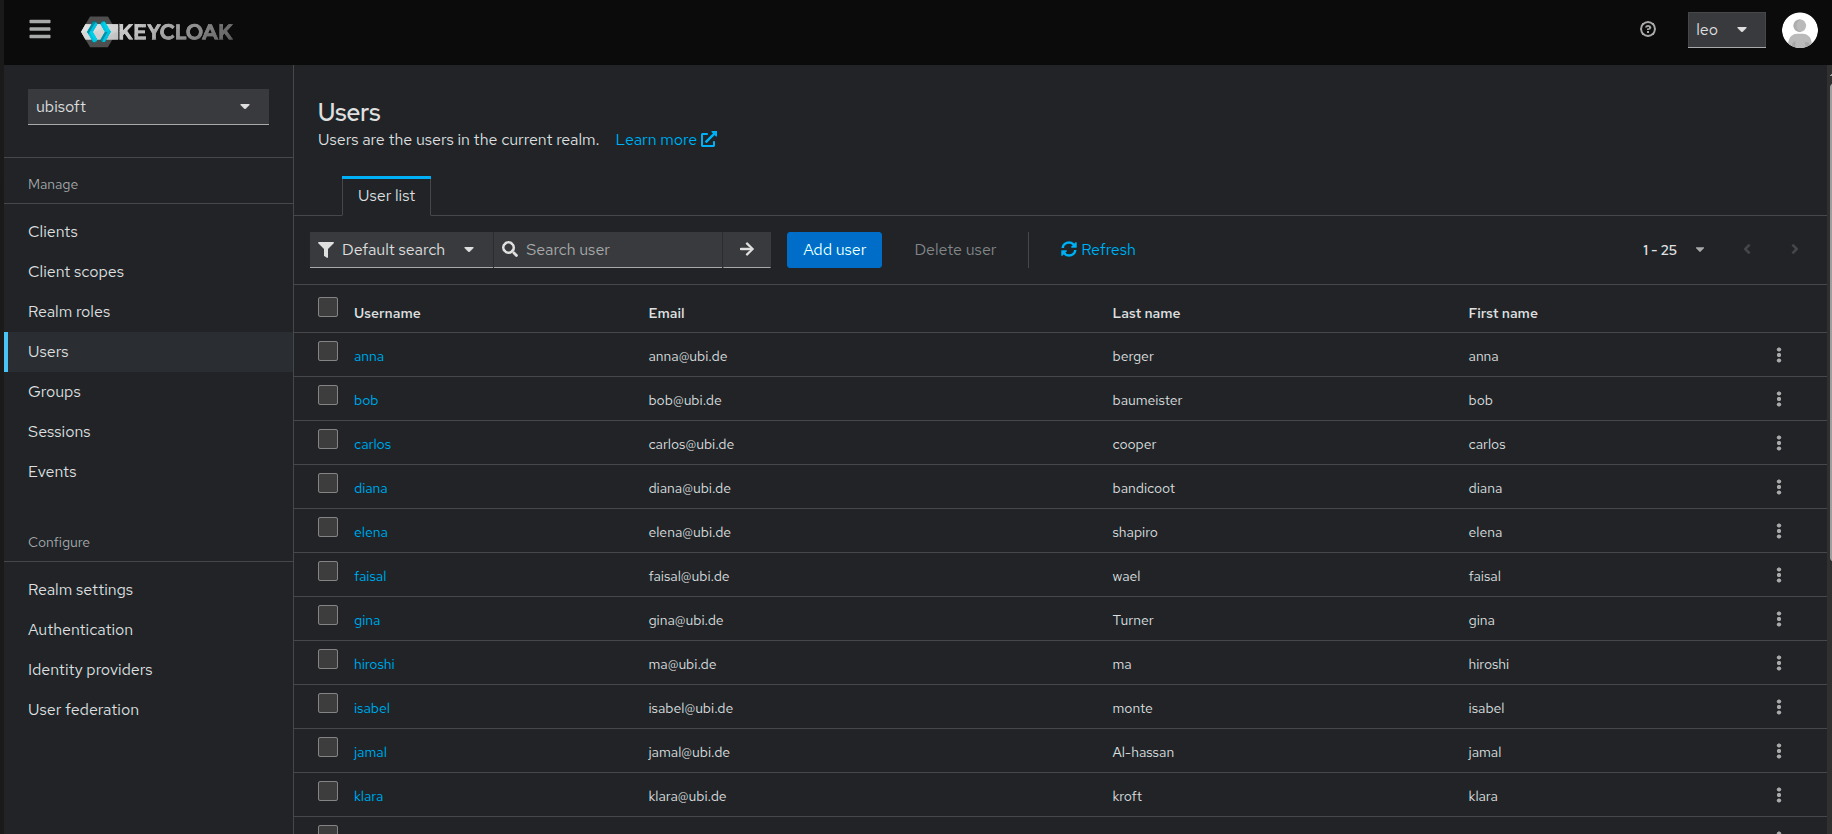
\includegraphics[scale=1.5, width=\linewidth]{screenshot011}
		\caption{Hier sieht man die generierten Benutzer für den Testfall}
		\label{fig:screenshot011}
	\end{figure}
	
	
	Es wurde zur Generierung der normalen Trainingsdaten zuvor vier Realms erstellt:
	
	\begin{itemize}
		\item ubisoft
		\item Nintendo
		\item Sega
		\item aws
	\end{itemize}
	
	Pro Realm erfolgt die Benutzeranmeldung über einen jeweils definierten Client.
	\\[0.5em]
	Im Realm \textit{ubisoft} wurden 25 synthetische Benutzer erstellt, deren Namen alphabetisch generiert wurden (jeder Buchstabe des Alphabets außer „X“ ist vertreten). Für diesen Realm wurde der Client \textit{ps3} angelegt. Dieser ist erforderlich, damit sowohl Administratoren Zugriff auf die User-Events erhalten als auch Benutzer sich über diesen Client authentifizieren können. Um sicherzustellen, dass während der Selenium-Tests nicht auf den Master-Realm zugegriffen wird, muss für den Client eine passende Redirect-URL definiert werden.
	\\[0.5em]
	In den weiteren Realms – \textit{Sega}, \textit{Nintendo} und \textit{aws} – wurden jeweils zehn Benutzer angelegt. Die zugehörigen Clients lauten: \textit{megadrive} (Sega), \textit{wii} (Nintendo) und \textit{aws-console} (aws).
	\\[0.5em]
	Jeder Realm verfügt über mindestens einen Administrator mit der Rolle \textit{realm-admin}. Ein Admin-Benutzer, der für einen bestimmten Client Benutzer anlegen oder verwalten möchte, benötigt darüber hinaus die Rollen \textit{manage-users} und \textit{view-events}. Wichtig ist hierbei, dass diese Rollen nicht direkt dem Benutzer zugewiesen werden, sondern dem jeweiligen Client. Der Grund dafür liegt in der Architektur von Keycloak: Clients besitzen eigene Zugriffsrechte, die ihnen bestimmte Operationen ermöglichen. So erlaubt die Rolle \textit{manage-users} dem Client, Benutzer im Realm programmatisch zu verwalten, während \textit{view-events} erforderlich ist, um Zugriff auf die Ereignisprotokolle zu erhalten – essenziell für Logging und Fehlersuche.
	\\[0.5em]
	Im Rahmen dieser Arbeit erzeugt ein Selenium-Test automatisch neue Benutzerkonten in Keycloak und weist ihnen jeweils ein Passwort zu. Diese Daten werden pro Realm einmalig in einer JSONL-Datei gespeichert, wobei Benutzername und Passwort gemeinsam als Schlüssel-Wert-Paar abgelegt werden.
	\\[0.5em]
	Damit sich die erzeugten Benutzer über die automatisierten Tests in Keycloak anmelden können, muss in der Konfiguration festgelegt werden, dass kein vollständiges Profil (Vorname, Nachname, E-Mail) erforderlich ist – andernfalls würde die Authentifizierung fehlschlagen.
	\\[0.5em]
	Darüber hinaus verfügen Clients über sogenannte Service Accounts – spezielle technische Benutzerkonten, die es ihnen ermöglichen, sich selbstständig zu authentifizieren, beispielsweise über den OAuth2 Client Credentials Grant. Die Service-Account-Rollen bestimmen dabei die verfügbaren Rechte. Ohne diese Rollen könnte der Client zwar eine Verbindung herstellen, hätte jedoch keinen Zugriff auf Benutzerverwaltung oder Logdaten. Die korrekte Konfiguration der Service-Account-Rollen ist daher zwingend notwendig, um im Hintergrund automatisiert operieren zu können.
	\\[0.5em]
	\begin{figure}[H]
		\centering
		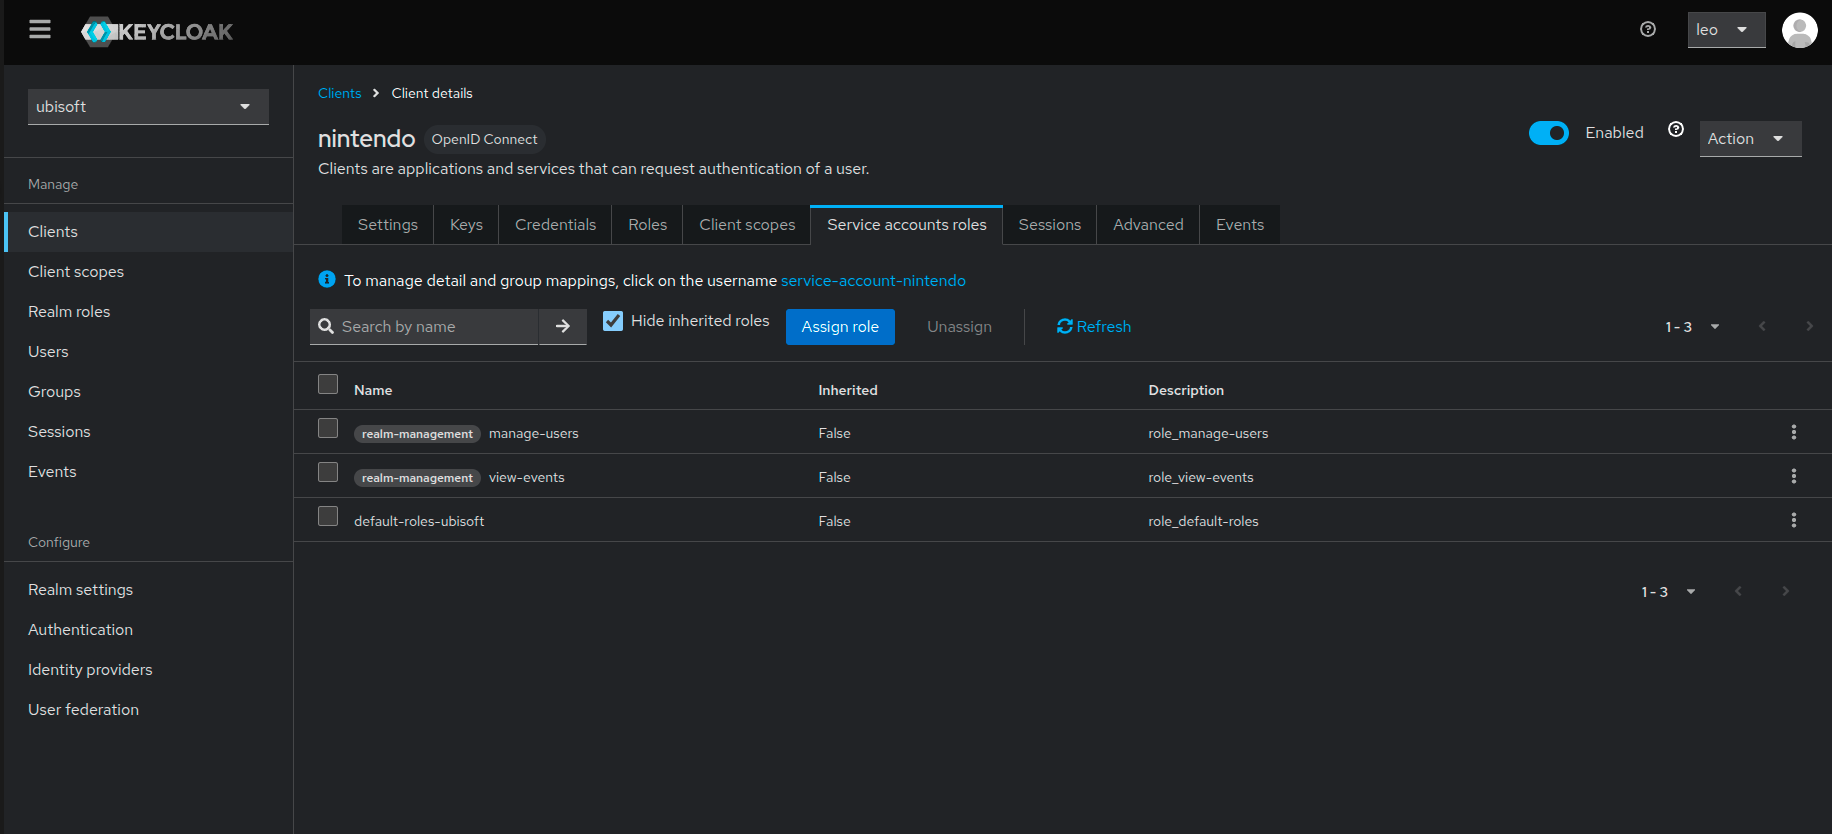
\includegraphics[width=0.9\linewidth]{screenshot012}
		\caption{Benötigte Rollen für den Client Nintendo}
		\label{fig:screenshot012}
	\end{figure}
	Ab einer bestimmten Menge an Trainingsdaten werden die generierten Benutzer im Rahmen des Selenium-Tests dazu gebracht, sich regulär anzumelden. Die dabei entstehenden sogenannten „gewöhnlichen“ Logs umfassen unter anderem Anmeldevorgänge und basieren auf realen firmeninternen Protokollen. Diese bestehen typischerweise aus den Event-Typen LOGIN, CLIENT\_LOGIN und CODE\_TO\_TOKEN.
	\\[0.5em]
	Folgende Aktivitäten gelten laut interner Log-Analyse als „typisch“:
	
	\begin{itemize}
		\item Anmeldung über Keycloak direkt
		\item Anmeldung über einen Client
		\item Token-Aktualisierung (Refresh Token)
		\item Abmeldung (Logout), auch nach Ablauf einer Session
		\item Fehlgeschlagene Logins (kommen häufiger vor)
	\end{itemize}
	
	Weitere Aktionen – wie das Anpassen des Benutzerprofils (z.B. E-Mail-Änderung, Passwort-Zurücksetzung), das Löschen eines Clients oder das Zuweisen von Rollen an andere Benutzer bzw. Clients – wurden in der Log-Generierung bewusst nicht automatisiert. Der Grund liegt in der vergleichsweise hohen Komplexität und der geringen Häufigkeit solcher Vorgänge. Da Keycloak primär als SSO-Dienst genutzt wird, wäre eine regelmäßige Durchführung solcher Aktionen im automatisierten Testkontext unrealistisch und würde die Aussagekraft der „normalen“ Logs verzerren.
	\\[0.5em]
	Stattdessen werden solche seltenen Aktionen manuell während des Testbetriebs von einzelnen Benutzern durchgeführt. Um dabei in die „Rolle“ eines anderen Benutzers zu schlüpfen, wird der Event-Typ IMPERSONATE verwendet. Die Verwendung von Impersonation während der automatisierten Testausführung wird vermieden, da sie eine potentielle Anomalie darstellt. Ziel ist es, lediglich gelegentlich und gezielt ungewöhnliche Aktionen zu erzeugen – etwa eine Passwort- oder E-Mail-Änderung, das Anlegen oder Löschen eines Benutzers oder das Zuweisen von Rollen. Dies reduziert den manuellen Aufwand bei der Erzeugung seltener Ereignisse, ohne die Gesamtdatenbasis zu verzerren.
	\\[0.5em]
	Pro Tag werden insgesamt 15 Sessions durchgeführt, wobei jede Session durch den häufigen Einsatz von Refresh Tokens mindestens zehn Einträge im Log erzeugt. Die Sitzungsdauer wird dabei durch die Konfiguration des jeweiligen Realms bestimmt. Aus praktischer Erfahrung ergibt sich eine durchschnittliche Dauer von etwa 35 Minuten pro Session – realistisch im Rahmen von 10 Minuten bis zu einer Stunde. So können pro Tag zwischen 2.500 und 5.000 Log-Einträge erzeugt werden.
	\\[0.5em]
	Zwar ließen sich innerhalb von fünf Tagen theoretisch bis zu 25.000 Log-Ereignisse erzeugen, jedoch ist der zeitliche Abstand zwischen den Sessions begrenzt. Ereignisse, die typischerweise erst nach längerer Zeit auftreten, fehlen somit in der Testbasis. Eine spätere Erweiterung ist möglich, jedoch wurde aufgrund der Bearbeitungsfrist beschlossen, die Generierung auf fünf aufeinanderfolgende Tage zu konzentrieren. Die Sessions werden dabei parallel ausgeführt.
	\\[0.5em]
	Da sämtliche Tests auf demselben Rechner stattfinden, ist die Quell-IP-Adresse für alle Benutzer identisch. Dies könnte bei längerem Training als Anomalie erkannt werden. Daher wird die IP-Adresse vor der Weiterverarbeitung aus den Events entfernt. Diese Maßnahme reduziert zwar eine potenzielle Störquelle, verringert aber gleichzeitig auch die Datenvielfalt für das Modell.
	\\[0.5em]
	Nichtsdestotrotz stellt dieses Verfahren eine vorteilhafte Methode zur Log-Generierung dar, da die erzeugten Ereignisse den realen Keycloak-Logs sehr nahekommen.
	
	\subsection{Mögliche Angriffszenarien nach CVE und CWE}
	Common Vulnerabilities and Exposures (CVE) stellt eine Auflistung bzw. Datenbank aller bekannten Sicherheitslücken in einem System dar. Für Keycloak existieren ebenfalls zahlreiche dokumentierte Schwachstellen \footnote{\url{https://cve.mitre.org/cgi-bin/cvekey.cgi?keyword=keycloak}}.
	\\[0.5em]
	CVEs bieten jedoch keine Lösungen an, sondern dienen der transparenten und neutralen Information über die Art, Ursache und mögliche Auswirkungen der jeweiligen Sicherheitslücke. Jede CVE erhält eine eindeutige Identifikationsnummer, eine Kurzbeschreibung sowie (sofern verfügbar) Angaben zur betroffenen Softwareversion. Die Dokumentation erfolgt weltweit durch Organisationen, Forschungseinrichtungen und unabhängige Sicherheitsforscher.
	\\[0.5em]
	Common Weakness Enumeration (CWE) hingegen beschreibt systematisch bekannte Schwachstellenmuster (Weaknesses), die potenziell zu Sicherheitslücken führen können. Während CVEs auf bereits konkret ausgenutzte oder gefundene Schwachstellen hinweisen, beschreibt CWE eher abstrakte Klassen von Fehlern, wie z.,B. „unzureichende Rechteprüfung“ oder „unsichere Tokenverarbeitung“. Beide Kataloge sind essentiell, um systematische Sicherheitstests zu entwerfen und zu interpretieren.
	\\[0.5em]
	Viele der genannten Probleme wurden zwar schon gelöst, jedoch häufen sich die Probleme von Jahr zu Jahr.
	Im Rahmen dieser Arbeit wurden mit Hilfe von Selenium gezielt sicherheitsrelevante Szenarien gegen Keycloak getestet und simuliert. Dabei lassen sich die folgenden Fälle konkreten CVE- und CWE-Einträgen zuordnen:

	\begin{itemize}
		\item \textbf{Privilege Escalation Test:}
		Bei diesem Test wurde überprüft, ob sich ein normaler Benutzer unbefugt Zugriff auf administrative Bereiche verschaffen kann. Die Logik entspricht dem bekannten Schwachstellenmuster \textbf{CWE-269: Improper Privilege Management}. In Bezug auf Keycloak wurde eine vergleichbare Schwachstelle mit \textbf{CVE-2019-10160} dokumentiert, bei der Benutzer durch unzureichende Prüfung ihrer Rollen Zugriff auf administrative Endpunkte erhalten konnten.
		\item \textbf{Token Manipulation Test:}  
		In diesem Test wurde ein gültiges OAuth2 Access Token manipuliert (z.\,B. durch Abschneiden und Ändern von Zeichen), um zu prüfen, ob das System die Signaturprüfung korrekt durchführt. Die zugrundeliegende Schwachstelle ist unter \textbf{CWE-347: Improper Verification of Cryptographic Signature} klassifiziert. Eine konkrete Verwundbarkeit, bei der ein ähnlicher Fall auftrat, ist \textbf{CVE-2020-13957}, bei dem manipulierte Tokens fälschlicherweise akzeptiert wurden.
		\item \textbf{Denial of Service (DoS) Test:}  
		Mittels zahlreicher, aufeinanderfolgender Anfragen wurde versucht, das System durch Last zu destabilisieren. Diese Art der Schwachstelle fällt unter \textbf{CWE-400: Uncontrolled Resource Consumption}. Eine reale CVE mit Bezug auf Keycloak ist \textbf{CVE-2021-41117}, bei der durch komplexe Gruppenrollenstrukturen ein ressourcenintensiver Zustand ausgelöst werden konnte, was ebenfalls zu einem DoS führen konnte.
	\end{itemize}
	
	Diese Tests orientieren sich an bekannten Sicherheitslücken und dienen dazu, die Robustheit des Systems unter realistischen Angriffsbedingungen zu validieren. Da CVE- und CWE-Datenbanken bewusst keine vollständigen Exploitbeschreibungen enthalten, musste im Rahmen der Simulation eine technische Interpretation der Schwachstellen erfolgen.
	
	Des weiteren werden noch folgende Angriffsszenarien durchgespielt, welche auch bei den generierten Logs durchgespielt wurden:
	
	\begin{itemize}
		\item \textbf{Session Hijacking:}  Missbrauch einer Session jemand anderes
		\item \textbf{Account Sabotage:}  Viele,Wichtige Ressourcen werden gelöscht oder verändert oder zugegriffen
		\item \textbf{Brute Force Attacke} 
	\end{itemize}
	
	\subsection{Selenium-Tests zur Erzeugung der Angriffsszenarien}
	
	Auch für die Selenium-Tests wurden die Angriffsszenarien wie in den generierten Logs umgesetzt.
	Für jeden Test, bzw. Angriffszenario wurde ein Ablauf konstruiert.
	Für den Fall einer \textbf{"Privilege Escalation"} wurde folgender Fall konstruiert:
	\\[0.5em]
	Im Ersten Fall versucht ein Nicht-Admin durch die Admin-Url zur Ansicht des Admins in Keycloak zu gelangen. Die würde schon fehlschlagen, wenn sich der Benutzer mit normalen Daten anmeldet.
	\\[1.0em]
	Der zweite Fall ist, dass der Admin selbst einem Benutzer zu viele Rechte gibt, oder bzw. der Benutzer selbst ist, nur eben hat der Benutzer die Admin-Credentials in Erfahrung gebracht:
	\\[0.5em]
	1. Man loggt sich in Keycloak direkt als der jeweilige Admin des zugehörigen Realms ein, (z.B. loggt sich Admin Anna in Realm Ubisoft ein).
	\\[0.5em]
	2. Admin geht zum Tab "users" und klickt auf den jeweiligen Benutzer, welcher zu viele Rechte erhalten soll
	\\[0.5em]
	3. Man klickt auf das Feld "Role Mapping"
	\\[0.5em]
	4. Es wird auf den Button 'Assign Role' gedrückt
	\\[0.5em]
	5. Sensible Rollen werden dem Benutzer zugefügt (z.B. "realm-admin")
	\\[0.5em]
	6. Man klickt auf den Button  'assign'
	\\[1.0em]
	Für den Fall \textbf{'Account Sabotage'} wurde folgendes Vorgehen entschieden:
	\\[0.5em]
	1. Man meldet sich an als Admin
	\\[0.5em]
	2. Als Admin werden viele Instanzen auf einmal gelöscht: Ein Client mit all seinen Benutzern
	\\[0.5em]
	Für den letzten Fall versucht ein gewöhnlicher Benutzer ständig Zugriff auf eine Ressource zu ergattern, die er nicht haben dürfte.
	\\[1.0em]
	Für den Fall \textbf{’Session Hijacking’} wurde folgendes Vorgehen konstruiert:
	\\[0.5em]
	1. Ein Angreifer loggt sich mit gültigen Zugangsdaten eines legitimen Benutzers in das System ein.
	\\[0.5em]
	2. Der Angreifer liest die Session-Cookies bzw. die Sitzungstoken des eingeloggten Benutzers aus.
	\\[0.5em]
	3. In einem zweiten Browser oder einer neuen Session werden diese Cookies übernommen und gesetzt.
	\\[0.5em]
	4. Der Angreifer ruft mit der übernommenen Sitzung eine geschützte Ressource auf, die nur dem legitimen Benutzer zugänglich sein sollte.
	\\[0.5em]
	5. Dadurch wird die aktive Benutzersitzung übernommen und unautorisierter Zugriff auf geschützte Bereiche ermöglicht.
	\\[1.0em]
	Für den Fall \textbf{"Token Manipulation"} wurde folgendes Vorgehen konstruiert:
	\\[0.5em]
	1. Ein Benutzer loggt sich mit gültigen Zugangsdaten im System ein.
	\\[0.5em]
	2. Das gültige Access-Token des Benutzers wird ermittelt.
	\\[0.5em]
	3. Das Token wird absichtlich verändert (z.B. durch Verfälschung der letzten Zeichen).
	\\[0.5em]
	4. Mit dem manipulierten Token wird eine Anfrage an die geschützte Admin-API gesendet.
	\\[0.5em]
	5. Das System sollte die Anfrage ablehnen und einen 401 Unauthorized-Status zurückgeben, um die Token-Manipulation zu erkennen.
	
	\section{Durchführung des Trainings}
	\section{Ergebnisse}
	\section{Diskussion}
	\section{Fazit}
	\section{Ausblick}
\newpage	
\bibliographystyle{unsrt}
\bibliography{quellen} 
\newpage 
\renewcommand{\notesname}{Fußnotenverzeichnis}
\renewcommand{\enoteformat}{\rightskip0pt\leftskip0pt\vspace{0.5em}\noindent\makebox[2em][l]{\theenmark}}
\theendnotes
\end{document}